% ===========================================================================
% Detecting Face-Swap Deepfakes by Verifying Skeletal Gait Dynamics
%
% Build (from paper/):  latexmk -pdf deepfake_paper.tex
%
% Figures 1-4 are conceptual diagrams generated outside this repository; see
% ../figures/GEMINI_PROMPTS.md. Until those PNGs are dropped into ../figures/,
% the \concept macro renders a labelled placeholder box so the document still
% compiles. Figures 5-11 are produced from the evaluation artefacts by
% ../scripts/generate_figures/generate_all.py.
% ===========================================================================

\documentclass[journal]{IEEEtran}

\usepackage[utf8]{inputenc}
\usepackage[T1]{fontenc}
\usepackage{amsmath,amssymb,amsfonts}
\usepackage{graphicx}
\usepackage{booktabs}
\usepackage{multirow}
\usepackage{array}
\usepackage{algorithm}
\usepackage{algorithmic}
\usepackage{xcolor}
\usepackage{url}
\usepackage{cite}

\graphicspath{{../figures/}{./}}

\hyphenation{deep-fake deep-fakes bio-mech-an-i-cal}

% Placeholder-tolerant include for the conceptual diagrams.
% #1 = path, #2 = width, #3 = short human-readable description
\newcommand{\concept}[3]{%
  \IfFileExists{#1}{\includegraphics[width=#2]{#1}}{%
    \setlength{\fboxsep}{7pt}%
    \fbox{\parbox[c][24mm][c]{\dimexpr#2-2\fboxsep-2\fboxrule\relax}{%
      \centering\footnotesize
      \textsc{figure placeholder}\\[3pt]
      #3\\[3pt]
      \textit{generation prompt in} \texttt{diagrams/GEMINI\_PROMPTS.md}}}}}

\newcommand{\tabhead}[1]{\textbf{#1}}

\begin{document}

\title{Detecting Face-Swap Deepfakes by Verifying\\Skeletal Gait Dynamics}

\author{Arhaan~Penwala,
        Abhishek~Arun~Raja~K,
        Aditya~Bharti,
        and~Vibhav~Sharma% <-this % stops a space
\thanks{A. Penwala (23BRS1155), A. Arun Raja K (23BRS1152), A. Bharti
(23BRS1199), and V. Sharma (23BPS1158) are with the School of Computer Science
and Engineering, Vellore Institute of Technology, Chennai Campus, India.}
\thanks{The GaitDeepfake-13 dataset supporting this work is available on IEEE
DataPort (DOI: 10.21227/ngh5-b637) and the evaluation code at
\protect\url{https://github.com/Arhaan-P/DeepFake-Detection}.}}

\markboth{IEEE Transactions on Biometrics, Behavior, and Identity Science}%
{Penwala \MakeLowercase{\textit{et al.}}: Detecting Face-Swap Deepfakes by Verifying Skeletal Gait Dynamics}

\maketitle

% ===========================================================================
\begin{abstract}
Face-swap deepfake generators synthesise a face and composite it back into an
otherwise unmodified frame. The body they leave behind still walks the way the
source person walks. We exploit this asymmetry directly: rather than searching
for artefacts inside the manipulated region, we verify the claimed identity
against the one signal the generator never touches. Given a video and a claimed
identity, our system extracts a 78-dimensional skeletal gait descriptor per
frame---hip-centred three-dimensional coordinates, six joint flexion angles and
frame-to-frame velocities over 12 biomechanically selected MediaPipe
landmarks---and classifies the per-timestep discrepancy between the observed
sequence and the claimed identity's enrolled signature using a temporal
convolutional verification network. We evaluate on GaitDeepfake-13, a
13-subject corpus of 66 walking videos expanded to 1{,}056 by a
16$\times$ augmentation pipeline, under strict leave-one-subject-out
cross-validation in which every video of the held-out subject, augmented or
not, is withheld from training. Over 2{,}240 pooled verification pairs the
system attains a pooled ROC-AUC of $94.95\%$ (per-fold $95.10\% \pm 3.08\%$),
accuracy $87.04\% \pm 3.65\%$, F1 $87.12\% \pm 3.77\%$ and an equal error rate
of $12.27\% \pm 3.80\%$. Gradient-based attribution shows the decision resting
on shoulder countermotion and distal heel-strike and toe-off kinematics, and
shows joint angles carrying $1.94\times$ their proportional share of
attribution despite occupying only 6 of 78 input dimensions. On three
FaceFusion-generated face-swap clips, the system rejected the claimed identity
in all three cases and matched the true body source with similarity above
$0.9998$, an existence check consistent with the core hypothesis though too
small to be a powered claim. An ablation over 13 folds and 3 seeds finds that wiring a
CNN, BiLSTM or Transformer encoder onto the decision path costs $2.5$ to $5.9$
ROC-AUC points against this minimal design (all $p < 10^{-3}$, paired), while
removing the raw per-timestep comparison collapses performance to chance---so
the simplicity of the verification network is a result, not a concession. We
position the work as occupying an under-explored niche rather than an empty
one, and delimit it against the behavioural-biometric and whole-body motion
forensics literature.
\end{abstract}

\begin{IEEEkeywords}
Deepfake detection, gait analysis, behavioural biometrics, pose estimation,
identity verification, skeletal keypoints, media forensics, explainable AI.
\end{IEEEkeywords}

% ===========================================================================
\section{Introduction}
\label{sec:intro}

\IEEEPARstart{T}{he} dominant paradigm in video deepfake detection is to look
for evidence of manipulation inside the manipulated region. Detectors learn
blending boundaries, frequency-domain irregularities, warping residues and
temporal flicker in and around the face
crop~\cite{recce,multi_attn,ftcn,altfreezing,fsbi}. The paradigm is
productive, and it is also structurally fragile: it places the detector in
direct opposition to the generator's objective. Every improvement in synthesis
quality erodes precisely the signal the detector depends on, which is why
cross-dataset generalisation remains the field's most stubborn
problem---methods that approach saturation within a training corpus lose
substantial ground on unseen manipulations and unseen
generators~\cite{recce,ftcn,deepfake_eval}.

This paper takes the opposite stance. Instead of interrogating the region the
adversary controls, we interrogate a region the adversary does not modify at
all.

The observation is mechanical rather than statistical. Contemporary face-swap
pipelines---FaceFusion with InSwapper~\cite{facefusion,insightface},
SimSwap~\cite{simswap} and their descendants---detect a face, synthesise a
replacement, and composite it back through a mask confined to the facial
region. The torso, limbs, and background are carried through from the source
footage, modulo recompression. Consequently a face-swapped video of person $B$
built on footage of person $A$ contains $B$'s face and $A$'s \emph{gait}. Human
locomotion is constrained by skeletal proportion, mass distribution, and
individual motor control, and is a well-established biometric in its own
right~\cite{gaitgraph,gaitpt,gaitformer,perry_gait,winter_biomech}. The forgery
therefore carries, in plain sight, an identity signal that contradicts its own
claim.

\subsection{Problem Formulation}

We treat detection as identity verification rather than binary artefact
classification. Given a video $V$ and a claimed identity $I_c$ drawn from an
enrolled gallery, the system computes
\begin{equation}
f(V, I_c) \rightarrow
\begin{cases}
\textsc{authentic} & \text{if the gait in } V \text{ matches } I_c,\\
\textsc{deepfake}  & \text{otherwise.}
\end{cases}
\label{eq:problem}
\end{equation}

This framing carries a consequence worth stating plainly at the outset: the
system detects an \emph{identity inconsistency}, not the presence of synthesis.
It requires an enrolled reference for the claimed identity and it will not flag
a wholly synthetic person with no claimed identity. Section~\ref{sec:discussion}
returns to what this rules in and out.

\subsection{Contributions}

\begin{enumerate}
\item \textbf{A gait-based verification formulation of face-swap detection},
      with a threat model in which the discriminative signal lies structurally
      outside the generator's output support rather than inside it
      (Section~\ref{sec:method}).
\item \textbf{A difference-based temporal verification network} that classifies
      the per-timestep discrepancy between an observed gait sequence and an
      enrolled signature. Operating on explicit sequence differences rather
      than on distances between separately pooled embeddings avoids the
      representation collapse we encountered with a Siamese formulation on a
      corpus of this size (Section~\ref{sec:verifier}).
\item \textbf{A subject-disjoint evaluation} over 13 leave-one-subject-out
      folds and 2{,}240 verification pairs, reporting per-fold dispersion and
      two distinct operating points rather than a single aggregate figure
      (Sections~\ref{sec:setup}--\ref{sec:results}).
\item \textbf{Gradient-based attribution over the skeleton}, which finds the
      model attending to biomechanically sensible structures, and which
      quantifies the disproportionate value of the six joint-angle dimensions
      (Section~\ref{sec:explain}).
\item \textbf{An ablation that justifies the architecture by refuting the
      alternative.} Across 13 folds and 3 seeds, wiring the CNN, BiLSTM or
      Transformer stack onto the decision path costs $2.5$ to $5.9$ ROC-AUC
      points against the deployed model (all $p < 10^{-3}$, paired), and
      removing the raw per-timestep comparison collapses performance to
      chance. The minimal difference network is not a simplification we
      settled for; it is the best of the configurations tested
      (Section~\ref{sec:ablation-results}).
\end{enumerate}

% ===========================================================================
\section{Related Work}
\label{sec:related}

\subsection{Face-Based Deepfake Detection}

Detection of facial manipulation has converged on spatial artefact modelling,
temporal coherence modelling, or a hybrid. Multi-attentional
detection~\cite{multi_attn} treats forgery detection as fine-grained
classification, aggregating evidence from multiple attended regions.
RECCE~\cite{recce} learns a reconstruction of genuine faces and uses
reconstruction error as the forgery cue, explicitly targeting generalisation;
the paper's own framing is instructive, observing that earlier methods degrade
towards approximately $60\%$ AUC on unseen data, and reporting roughly $70.9\%$
cross-dataset AUC on Celeb-DF-v2 for its own approach. FTCN~\cite{ftcn} removes
spatial convolution capacity to force reliance on temporal incoherence,
reaching roughly $86$--$89\%$ AUC on Celeb-DF as a cross-dataset result.
AltFreezing~\cite{altfreezing} alternately freezes spatial and temporal weights
in a 3D ConvNet to balance both artefact families, reporting $89.5\%$
cross-dataset AUC on Celeb-DF. FSBI~\cite{fsbi} synthesises training forgeries
via frequency-enhanced self-blending.

The pattern across this literature is that in-corpus performance is close to
saturated while cross-corpus performance is not, and the gap is
generator-dependent. Our approach is complementary rather than competitive: it does not
examine the facial region at all, and so its failure modes are uncorrelated
with those of every method in this subsection.

\subsection{Skeleton-Based Gait Recognition}

Model-based gait recognition operates on pose sequences rather than
silhouettes, which confers robustness to clothing and carried objects.
GaitGraph~\cite{gaitgraph} applies graph convolution to skeleton sequences.
GaitPT~\cite{gaitpt} shows a hierarchical pose transformer reaching $82.6\%$
average accuracy on CASIA-B from skeletons alone. GaitFormer~\cite{gaitformer}
reports $92.5\%$ on CASIA-B after multi-task pretraining on a large
automatically-annotated corpus. GPGait~\cite{gpgait} targets cross-domain
generalisation from pose. Liao \emph{et al.}~\cite{liao_gait} incorporate human
prior knowledge into a model-based recogniser.

This body of work establishes that skeletal kinematics carry sufficient
identity information for recognition at scale. We inherit that premise and
redirect it: our task is not to recognise an unknown walker among many, but to
adjudicate a specific claimed identity, which is a verification problem with
its own metric conventions~\cite{iso19795}.

\subsection{Behavioural and Whole-Body Forgery Detection}

Behavioural biometrics entered deepfake detection with Agarwal
\emph{et al.}~\cite{agarwal2019}, who modelled correlations among facial action
units and head motion to build per-individual behavioural profiles, later
combining static facial and temporal behavioural
biometrics~\cite{agarwal2020} and subsequently extending beyond the face to
gestural and vocal mannerisms~\cite{agarwal_pnas}. More recently, attention has
moved to the whole body. Human Action CLIPs~\cite{humanactionclips} detects
AI-generated human motion. TT-DF~\cite{ttdf} provides a large-scale benchmark
for human body forgery detection exploiting pose and motion inconsistency.
Chapariniya \emph{et al.}~\cite{convkeypoints} identify people from
whole-body conversational keypoints, framed explicitly against face-reenactment
threats. Closest to the present work, DeAndres-Tame
\emph{et al.}~\cite{gaitfidelity} evaluate whether generative human-animation
models preserve gait identity cues, and find that they do not---an evaluation
study rather than a deployed detector, but one that independently supports the
premise this paper builds on.

\subsection{Positioning}

We state our position precisely, because a looser claim would not survive
contact with the literature above. Behavioural biometrics have been applied to
deepfake detection since 2019~\cite{agarwal2019}, and whole-body pose and
motion cues have been applied since at least 2024--2025
\cite{humanactionclips,ttdf,convkeypoints}. What remains under-explored, to our
knowledge, is the use of \emph{locomotion gait-cycle skeletal dynamics as the
primary discriminative feature} for verifying a claimed identity in a
face-swapped video, evaluated under subject-disjoint protocol against
generator-produced forgeries. The nearest work~\cite{gaitfidelity} measures
gait fidelity in generated animation without building a detector; the nearest
detectors~\cite{ttdf,humanactionclips} target whole-body synthesis rather than
face-swap, where the body is authentic and only the claim is false. We
therefore describe this as an under-explored niche, not a vacant one, and
Table~\ref{tab:comparison} is offered as positioning rather than as a
leaderboard.

% ===========================================================================
\section{Proposed Method}
\label{sec:method}

Fig.~\ref{fig:pipeline} gives an overview of the end-to-end verification
pipeline described in this section, from raw video to verdict.

\begin{figure*}[!t]
\centering
\concept{../figures/fig1_pipeline.png}{\textwidth}{%
  System pipeline: video and claimed identity $\rightarrow$ MediaPipe pose
  $\rightarrow$ 78-dim gait features $\rightarrow$ temporal normalisation
  $\rightarrow$ difference-based verification CNN $\rightarrow$ verdict.}
\caption{End-to-end verification pipeline. A walking video and a claimed
identity enter at the left; MediaPipe Pose yields 33 landmarks per frame, of
which 12 gait-relevant keypoints are retained and expanded into a
78-dimensional per-frame descriptor. Sequences are resampled to $T = 60$ frames
and z-score normalised using statistics computed on the training split only.
The verification network compares the resulting sequence against the claimed
identity's enrolled signature and emits a calibrated score, which the
Youden-optimal threshold $\tau^* = 0.7737$ converts into a verdict. Note that
the enrolled signature enters the network as a second input sequence, not as a
stored embedding.}
\label{fig:pipeline}
\end{figure*}

\subsection{Threat Model}
\label{sec:threat}

\begin{figure}[!t]
\centering
\concept{../figures/fig2_threat_model.png}{\columnwidth}{%
  Threat model: the generator rewrites only the face crop, so the forged
  video retains the source body's gait.}
\caption{The asymmetry the method exploits. A face-swap generator detects a
face, synthesises a replacement, and composites it back through a face-confined
mask; the torso, limbs and background of the source footage pass through
essentially unmodified. A forgery claiming to depict person~$B$ therefore
carries person~$A$'s gait. Because the generator never models locomotion, this
inconsistency is not an artefact that improved synthesis quality will remove---%
it is a structural property of face-region-only manipulation.}
\label{fig:threat}
\end{figure}

We assume an adversary who produces a face-swapped video: a genuine recording
of a source subject with a target subject's face composited into the facial
region, presented under the target's identity. The adversary may use any
face-swap model and any face-enhancement post-process, and may recompress the
result. The adversary does \emph{not} re-synthesise or retime body motion.

Under this model the detector's task reduces to Eq.~\ref{eq:problem}, and its
robustness has an unusual character: it is invariant to the quality of the face
swap, because it never observes the swapped region. Fig.~\ref{fig:threat}
illustrates the mechanism. Section~\ref{sec:discussion} discusses adversaries
who violate the final assumption.

\subsection{Dataset}
\label{sec:dataset}

Evaluation uses GaitDeepfake-13~\cite{gaitdeepfake13}, collected for this work.
Thirteen subjects were recorded walking at natural pace in controlled indoor
conditions, from frontal (F) and side (S) viewpoints, yielding 66 original
recordings at 30\,fps and 720p--1080p. Subjects were students aged approximately
19--25 of both sexes. Table~\ref{tab:dataset} summarises the corpus.

\begin{table}[!t]
\caption{Composition of the GaitDeepfake-13 Corpus}
\label{tab:dataset}
\centering
\begin{tabular}{ll}
\toprule
\tabhead{Property} & \tabhead{Value} \\
\midrule
Subjects (enrolled identities)   & 13 \\
Original recordings              & 66 (3--5 per subject) \\
After 16$\times$ augmentation    & 1{,}056 \\
Viewpoints                       & Frontal (F), side profile (S) \\
Frame rate / resolution          & 30\,fps / 720p--1080p \\
Sequence length                  & $T = 60$ frames ($\approx$2\,s) \\
Per-frame feature dimension      & 78 \\
Face-swapped test clips          & 3 (FaceFusion / InSwapper) \\
LOOCV verification pairs         & 2{,}240 (1{,}120 genuine) \\
\bottomrule
\end{tabular}
\end{table}

\subsubsection{Augmentation}
Each recording was expanded 16$\times$ ($66 \times 16 = 1{,}056$) by the
transformations in Table~\ref{tab:augmentation}. The design constraint was that
no transformation may alter the underlying skeletal trajectory. Photometric
operations (blur, brightness, contrast, colour jitter, grayscale, noise) change
pixels but not the pose MediaPipe recovers from them; geometric rotation is
capped at $10^{\circ}$ to avoid anatomically implausible configurations;
temporal operations exploit the approximate time-reversal symmetry and natural
speed variability of the gait cycle~\cite{shorten_survey,perry_gait}.

We note the limitation this implies. Augmentation multiplies the number of
training sequences but not the number of \emph{gaits}: the effective sample
size for a subject-level generalisation claim remains 13, and
Section~\ref{sec:threats} treats this accordingly.

\begin{table}[!t]
\caption{Augmentation Operations (16$\times$ Expansion)}
\label{tab:augmentation}
\centering
\small
\begin{tabular}{@{}clp{2.55cm}@{}}
\toprule
\tabhead{\#} & \tabhead{Operation} & \tabhead{Purpose} \\
\midrule
1  & Original                       & Baseline \\
2  & Horizontal flip                & Bilateral symmetry \\
3  & Gaussian blur (kernel 3--5)    & Codec / motion artefacts \\
4  & Brightness $-0.2$ to $-0.3$    & Low light \\
5  & Brightness $+0.2$ to $+0.3$    & Overexposure \\
6  & Contrast $+0.2$ to $+0.3$      & High-contrast scenes \\
7  & Colour jitter                  & Colour invariance \\
8  & Combined multi-augment         & Compound robustness \\
9  & Grayscale                      & Colour invariance \\
10 & Rotation left $5$--$10^{\circ}$  & Camera tilt \\
11 & Rotation right $5$--$10^{\circ}$ & Camera tilt \\
12 & Speed $0.8\times$              & Slow gait \\
13 & Speed $1.2\times$              & Fast gait \\
14 & Temporal reversal              & Gait time symmetry \\
15 & Zoom (crop and resize)         & Framing variation \\
16 & Gaussian noise injection       & Sensor noise \\
\bottomrule
\end{tabular}
\end{table}

\subsection{Pose Estimation and Feature Extraction}
\label{sec:features}

\subsubsection{Landmark Selection}
Pose is estimated with MediaPipe Pose Landmarker~\cite{mediapipe}
(\texttt{pose\_landmarker\_lite}, FP16, per-frame IMAGE mode, detection and
tracking confidence $0.5$), producing 33 three-dimensional landmarks per frame.
Of these we retain the 12 listed in Table~\ref{tab:landmarks} and shown in
Fig.~\ref{fig:keypoints}. The selection is driven by gait
biomechanics~\cite{perry_gait,whittle_gait,winter_biomech}: the lower-limb
chain from hip through knee, ankle, heel and foot index spans the events that
define the gait cycle---heel strike, stance, toe-off---while the shoulders
capture the trunk countermotion that balances angular momentum during
swing. Facial, elbow and wrist landmarks are discarded; the facial ones are
discarded on principle, since they lie inside the region the adversary controls.

Video-based pose estimation is accurate enough for this purpose. Stenum
\emph{et al.}~\cite{stenum2021} validated markerless video pose estimation
against a Vicon optical motion-capture system and reported mean absolute errors
of $4.0^{\circ}$, $5.6^{\circ}$ and $7.4^{\circ}$ for sagittal-plane hip, knee
and ankle angles respectively. We cite that result for the general claim it
supports---that video pose estimation agrees with laboratory motion capture to
within a few degrees---and note that it evaluated OpenPose rather than
MediaPipe, so it is corroborating rather than direct evidence for our
particular backend.

\begin{figure}[!t]
\centering
\concept{../figures/fig3_keypoints.png}{\columnwidth}{%
  The 12 retained MediaPipe landmarks on a body skeleton, with the 21
  discarded landmarks shown de-emphasised.}
\caption{The 12 gait keypoints retained from MediaPipe's 33 landmarks, shown on
the kinematic chain used to compute joint angles. Retained landmarks are the
bilateral shoulders, hips, knees, ankles, heels and foot indices; the discarded
landmarks---face, elbows, wrists and hands---are drawn de-emphasised. Discarding
the facial cluster is a design commitment rather than an economy: it is the
region a face-swap adversary controls, and admitting it would reintroduce
exactly the dependency this method exists to avoid.}
\label{fig:keypoints}
\end{figure}

\begin{table}[!t]
\caption{The 12 Retained Gait Landmarks}
\label{tab:landmarks}
\centering
\small
\begin{tabular}{@{}clcl@{}}
\toprule
\tabhead{Idx} & \tabhead{Landmark} & \tabhead{MP~ID} & \tabhead{Gait role} \\
\midrule
0  & Left shoulder    & 11 & Trunk countermotion \\
1  & Right shoulder   & 12 & Trunk countermotion \\
2  & Left hip         & 23 & Pelvic motion, CoM \\
3  & Right hip        & 24 & Pelvic motion, CoM \\
4  & Left knee        & 25 & Flexion kinematics \\
5  & Right knee       & 26 & Flexion kinematics \\
6  & Left ankle       & 27 & Foot placement, stride \\
7  & Right ankle      & 28 & Foot placement, stride \\
8  & Left heel        & 29 & Heel strike \\
9  & Right heel       & 30 & Heel strike \\
10 & Left foot index  & 31 & Toe-off \\
11 & Right foot index & 32 & Toe-off \\
\bottomrule
\end{tabular}
\end{table}

\subsubsection{The 78-Dimensional Descriptor}
For frame $t$ the descriptor concatenates three blocks,
\begin{equation}
\mathbf{f}_t = \left[\, \mathbf{c}_t \;\|\; \boldsymbol{\theta}_t \;\|\;
\mathbf{v}_t \,\right] \in \mathbb{R}^{78},
\end{equation}
composed as set out in Table~\ref{tab:features}.

\emph{Normalised coordinates} $\mathbf{c}_t \in \mathbb{R}^{36}$ are the 12
landmark positions re-expressed relative to the pelvis centre,
\begin{equation}
\hat{\mathbf{p}}_i^{(t)} = \mathbf{p}_i^{(t)} -
\tfrac{1}{2}\left(\mathbf{p}_{\text{L\_Hip}}^{(t)} +
\mathbf{p}_{\text{R\_Hip}}^{(t)}\right),
\quad i = 1,\dots,12,
\end{equation}
which removes translation and much of the scale variation induced by camera
distance~\cite{gaitgraph,gaitpt}.

\emph{Joint angles} $\boldsymbol{\theta}_t \in \mathbb{R}^{6}$ are the
three-point flexion angles at both knees, hips and ankles,
\begin{equation}
\theta_{abc} = \arccos\!\left(
\frac{(\mathbf{p}_a - \mathbf{p}_b) \cdot (\mathbf{p}_c - \mathbf{p}_b)}
{\lVert \mathbf{p}_a - \mathbf{p}_b \rVert \,
 \lVert \mathbf{p}_c - \mathbf{p}_b \rVert}\right),
\end{equation}
evaluated as $\theta(\text{hip},\text{knee},\text{ankle})$,
$\theta(\text{shoulder},\text{hip},\text{knee})$ and
$\theta(\text{knee},\text{ankle},\text{foot})$ bilaterally. Angles are
scale-free by construction and encode biomechanical constraint directly
\cite{perry_gait,whittle_gait}.

\emph{Velocities} $\mathbf{v}_t = \mathbf{c}_t - \mathbf{c}_{t-1} \in
\mathbb{R}^{36}$ are first-order differences, with $\mathbf{v}_1 = \mathbf{0}$,
capturing the rate structure of the gait cycle~\cite{phinyomark}.

\begin{table}[!t]
\caption{Composition of the 78-Dimensional Per-Frame Descriptor}
\label{tab:features}
\centering
\footnotesize
\begin{tabular}{@{}lccl@{}}
\toprule
\tabhead{Block} & \tabhead{Dims} & \tabhead{Index} & \tabhead{Content} \\
\midrule
Norm. coordinates & 36 ($12\times3$) & $[0{:}36)$  & Hip-centred $(x,y,z)$ \\
Joint angles      & 6                & $[36{:}42)$ & Knee/hip/ankle flexion \\
Velocities             & 36 ($12\times3$) & $[42{:}78)$ & $\Delta$ coordinates \\
\midrule
\textbf{Total}         & \textbf{78}      &             & \\
\bottomrule
\end{tabular}
\end{table}

\subsubsection{Temporal and Statistical Normalisation}
Sequences are resampled to $T = 60$ frames: longer sequences are uniformly
subsampled, shorter ones zero-padded, and clips yielding fewer than 10 valid
frames are rejected. At 30\,fps, 60 frames span roughly two seconds, covering
one to two complete gait cycles~\cite{perry_gait}. Each of the 78 dimensions is
then z-score normalised,
$\hat{f}_j = (f_j - \mu_j)/\max(\sigma_j, 10^{-6})$,
which is necessary because the blocks occupy incommensurate
scales~\cite{lecun_efficient}. Under LOOCV, $\mu_j$ and $\sigma_j$ are
recomputed inside every fold.

We record one protocol detail for reproducibility. The evaluation script that
produced our headline LOOCV figures normalises the held-out subject using that
subject's own statistics rather than the training split's---a transductive
choice, and not the one a strict reading of the protocol would imply. We
measured what it is worth by running the deployed model both ways across all 13
folds: training statistics yield $94.67\% \pm 3.06\%$ ROC-AUC against
$94.97\% \pm 2.90\%$ for the shipped behaviour, a difference of $0.30$ points
that is not statistically significant ($p = 0.73$, paired, $n = 13$). The
headline result is therefore insensitive to this choice, and all ablation
comparisons in Section~\ref{sec:ablation-results} use training statistics
throughout.

\subsection{Identity Enrolment}
\label{sec:enrollment}

Each identity $I$ is enrolled by averaging the descriptors of its original
(non-augmented) recordings per timestep,
\begin{equation}
\bar{\mathbf{f}}_t^{(I)} = \frac{1}{|V_I|}\sum_{v \in V_I} \mathbf{f}_t^{(v)},
\qquad t = 1,\dots,60,
\end{equation}
yielding a $60 \times 78$ signature stored per subject. Averaging across
recordings suppresses per-take noise while preserving the subject's
characteristic temporal profile. The signature is used as a full sequence, not
collapsed to a vector---the verification network consumes it as a second input
stream.

\subsection{Verification Network}
\label{sec:verifier}

\begin{figure*}[!t]
\centering
\concept{../figures/fig4_architecture.png}{\textwidth}{%
  Architecture: the verification path (pairwise comparison $\rightarrow$
  temporal CNN $\rightarrow$ softmax) and the separate auxiliary embedding
  path (GaitEncoder $\rightarrow$ DualPathTemporalModel).}
\caption{Network architecture as trained. The lower lane is the verification
path: the observed and claimed sequences are combined into a 234-channel
per-timestep comparison tensor, passed through a three-layer temporal CNN,
pooled and classified. The upper lane---a residual 1D CNN encoder feeding a
parallel BiLSTM and Transformer---produces a 128-dimensional gait embedding
used for enrolment analysis and diagnostics. The two lanes do not join: under
the cross-entropy objective applied to the softmax output, $133{,}058$
parameters lie on the verification path and $715{,}556$ do not.
Section~\ref{sec:aux} states the consequences of this separation, and
Section~\ref{sec:threats} treats it as a threat to validity.}
\label{fig:architecture}
\end{figure*}

The verification network classifies the discrepancy between the observed
sequence $\mathbf{V} \in \mathbb{R}^{T \times 78}$ and the claimed identity's
signature $\mathbf{C} \in \mathbb{R}^{T \times 78}$ directly, without first
reducing either to a pooled embedding.

\subsubsection{Pairwise Comparison Tensor}
Three per-timestep comparison signals are concatenated,
\begin{equation}
\mathbf{F} = \left[\, (\mathbf{V}-\mathbf{C}) \;\|\;
|\mathbf{V}-\mathbf{C}| \;\|\;
(\mathbf{V} \odot \mathbf{C}) \,\right] \in \mathbb{R}^{T \times 234},
\end{equation}
where the signed difference localises \emph{where} and \emph{in which
direction} the sequences diverge, the absolute difference supplies magnitude
invariant to sign, and the elementwise product responds where the two agree.

\subsubsection{Temporal Classifier}
$\mathbf{F}$ is transposed to channel-first order and passed through three 1D
convolutional stages with decreasing receptive fields
($234 \rightarrow 64$, $k=7$; $64 \rightarrow 64$, $k=5$;
$64 \rightarrow 32$, $k=3$), each with batch normalisation and ReLU, and
dropout on the first two. Global average pooling over time yields a
32-dimensional summary, which a two-layer MLP maps to two logits. The verdict
score is $P(\textsc{authentic}) = \mathrm{softmax}(\cdot)_1$.
Algorithm~\ref{alg:verify} states the forward pass.

\begin{algorithm}[!t]
\caption{Difference-Based Verification Forward Pass}
\label{alg:verify}
\begin{algorithmic}[1]
\REQUIRE Observed $\mathbf{V} \in \mathbb{R}^{B\times T\times 78}$,
         claimed $\mathbf{C} \in \mathbb{R}^{B\times T\times 78}$
\STATE $\mathbf{D} \leftarrow \mathbf{V} - \mathbf{C}$
\STATE $\mathbf{F} \leftarrow [\mathbf{D} \,\|\, |\mathbf{D}| \,\|\,
        \mathbf{V}\odot\mathbf{C}] \in \mathbb{R}^{B\times T\times 234}$
\STATE $\mathbf{F} \leftarrow \mathrm{permute}(\mathbf{F})
        \in \mathbb{R}^{B\times 234\times T}$
\STATE $\mathbf{F} \leftarrow \mathrm{ReLU}(\mathrm{BN}(
        \mathrm{Conv1D}_{234\rightarrow 64,\,k=7}(\mathbf{F})))$; dropout
\STATE $\mathbf{F} \leftarrow \mathrm{ReLU}(\mathrm{BN}(
        \mathrm{Conv1D}_{64\rightarrow 64,\,k=5}(\mathbf{F})))$; dropout
\STATE $\mathbf{F} \leftarrow \mathrm{ReLU}(\mathrm{BN}(
        \mathrm{Conv1D}_{64\rightarrow 32,\,k=3}(\mathbf{F})))$
\STATE $\mathbf{z} \leftarrow \mathrm{AdaptiveAvgPool1D}(\mathbf{F})
        \in \mathbb{R}^{B\times 32}$
\STATE $\boldsymbol{\ell} \leftarrow
        \mathrm{Linear}_{32\rightarrow 2}(\mathrm{Dropout}(\mathrm{ReLU}(
        \mathrm{Linear}_{32\rightarrow 32}(\mathbf{z}))))$
\RETURN $P(\textsc{authentic}) = \mathrm{softmax}(\boldsymbol{\ell})_1$
\end{algorithmic}
\end{algorithm}

\subsubsection{Why Differences Rather Than Embedding Distances}
Our initial design followed the standard Siamese template: encode both
sequences with shared weights, pool to embeddings, and score their distance. On
this corpus it collapsed---the encoder converged to a near-constant embedding,
driving all pairwise distances towards a single value and the classifier
towards the majority prediction. With 13 identities and a per-timestep
signature that is itself an average of few recordings, the pooling step
discards precisely the fine temporal structure that separates individuals.
Comparing sequences before pooling avoids the failure: the discriminative
information is preserved at full temporal resolution and the pooling that does
occur happens after the comparison, on evidence rather than on identity.

\subsection{Auxiliary Representation Branch}
\label{sec:aux}

The trained checkpoint also contains a representation branch, retained from the
Siamese design and used for enrolment analysis and diagnostics: a residual 1D
CNN encoder (\textsc{GaitEncoder}, $78 \rightarrow 64 \rightarrow 128$ with two
residual blocks~\cite{resnet}) feeding a dual-path temporal model
(\textsc{DualPathTemporalModel}) whose BiLSTM~\cite{lstm} ($h=64$, one layer,
bidirectional) and Transformer encoder~\cite{vaswani} ($d_{\text{model}}=128$,
4 heads, 2 layers, $d_{\text{ff}}=512$, GELU~\cite{gelu}, pre-LayerNorm
\cite{preln}, sinusoidal positional encoding) are fused by an MLP into a
128-dimensional embedding. Linear layers use Xavier
initialisation~\cite{glorot_init} and convolutions He
initialisation~\cite{he_init}. Table~\ref{tab:config} gives the configuration
as trained.

We must be explicit about this branch's role, because the distinction affects
how the results in Section~\ref{sec:results} should be read. Under the
cross-entropy objective applied to the verification logits, gradients reach
only the pairwise-comparison path. The representation branch produces an
embedding that is not consumed by the classifier and receives no learning
signal from the training objective. Of the model's $848{,}614$ parameters,
$133{,}058$ ($15.7\%$) lie on the decision path.

All quantitative results in this paper are therefore properties of the
difference-based verification network, not of the CNN--BiLSTM--Transformer
stack. Section~\ref{sec:ablation-results} takes the further step of asking
whether that stack \emph{should} be connected, and finds that it should not:
every configuration that routes it onto the decision path is significantly
worse than leaving it off. Fig.~\ref{fig:architecture} draws the separation
explicitly.

\begin{table}[!t]
\caption{Model Configuration as Trained}
\label{tab:config}
\centering
\footnotesize
\begin{tabular}{@{}llr@{}}
\toprule
\tabhead{Component} & \tabhead{Setting} & \tabhead{Params} \\
\midrule
\multicolumn{3}{@{}l}{\emph{Verification path (trained)}}\\
Comparison tensor      & $78 \times 3 = 234$ channels & --- \\
Temporal CNN           & $k = 7, 5, 3$; $64,64,32$ ch. & 131{,}936 \\
Classifier MLP         & $32 \rightarrow 32 \rightarrow 2$ & 1{,}122 \\
\midrule
\multicolumn{3}{@{}l}{\emph{Auxiliary branch (not on decision path)}}\\
GaitEncoder            & $78 \rightarrow 64 \rightarrow 128$ & 129{,}600 \\
DualPathTemporalModel  & BiLSTM $h{=}64$; Trans. $d{=}128$ & 546{,}304 \\
Identity verifier head & $128$, hidden $64$ & 31{,}266 \\
Standalone classifier  & $128 \rightarrow 64 \rightarrow 2$ & 8{,}386 \\
\midrule
\multicolumn{2}{@{}l}{\textbf{Total}} & \textbf{848{,}614} \\
\multicolumn{2}{@{}l}{\textbf{On decision path}} & \textbf{133{,}058} \\
\bottomrule
\end{tabular}
\end{table}

\subsection{Training}
\label{sec:training}

Training pairs are sampled with a $50/50$ balance: half pair a video with its
own identity's signature (label \textsc{authentic}), half with a uniformly
sampled different identity's signature (label \textsc{deepfake}). This
simulates the identity-mismatch condition a face swap induces, and prevents the
degenerate constant-prediction solution~\cite{facenet}. Optimisation uses
AdamW~\cite{adamw} at $10^{-3}$ with weight decay $10^{-4}$, batch size 16,
gradient-norm clipping at $1.0$~\cite{pascanu}, dropout
$0.1$~\cite{dropout}, and \texttt{ReduceLROnPlateau} (factor $0.5$, patience
7). Early stopping monitors validation accuracy with patience 20 and
$\delta_{\min} = 10^{-3}$~\cite{prechelt}. The loss is class-weighted
cross-entropy on the two verification logits. Table~\ref{tab:training}
summarises the settings; the single-split reference model reached $93.92\%$
validation accuracy at epoch 46, against $98.38\%$ training accuracy.

\begin{table}[!t]
\caption{Training Configuration}
\label{tab:training}
\centering
\footnotesize
\begin{tabular}{@{}lll@{}}
\toprule
\tabhead{Parameter} & \tabhead{Value} & \tabhead{Rationale} \\
\midrule
Optimiser        & AdamW                & Decoupled decay~\cite{adamw} \\
Learning rate    & $1\times10^{-3}$     & Adam default~\cite{adam} \\
Weight decay     & $1\times10^{-4}$     & Moderate regularisation \\
Scheduler        & Plateau, $\times0.5$ & Patience 7 \\
Grad. clipping   & $\lVert g \rVert \le 1.0$ & Stability~\cite{pascanu} \\
Dropout          & $0.1$                & Small corpus~\cite{dropout} \\
Batch size       & 16                   & $\sim$1k samples~\cite{masters_batch} \\
Max epochs       & 50 (LOOCV: 30)       & With early stopping \\
Early stopping   & Patience 20          & \cite{prechelt} \\
Loss             & Weighted CE          & Two-class logits \\
Pair sampling    & 50/50 balanced       & \cite{facenet} \\
Hardware         & NVIDIA RTX 3050, 6\,GB & CUDA 12.4 \\
\bottomrule
\end{tabular}
\end{table}

% ===========================================================================
\section{Experimental Setup}
\label{sec:setup}

\subsection{Leave-One-Subject-Out Cross-Validation}

The primary protocol is 13-fold leave-one-subject-out cross-validation
(Algorithm~\ref{alg:loocv}). In fold $k$, every recording of subject $s_k$---%
original and all 15 augmentations---is withheld, normalisation statistics are
recomputed from the remaining 12 subjects, and a model is trained from scratch
for 30 epochs before being evaluated on the held-out subject's pairs.

Subject-level rather than video-level partitioning is not a refinement but a
requirement. Because augmented clips are derived from originals, a video-level
split would place 15 near-duplicates of a test clip into training and produce
an estimate with no bearing on unseen subjects. LOOCV is the appropriate
protocol for small-cohort biometric evaluation~\cite{iso19795}, with the caveat
that its variance is high at this cohort size~\cite{varoquaux_small}. The full
13-fold procedure completed in 1{,}228\,s.

\begin{algorithm}[!t]
\caption{Leave-One-Subject-Out Evaluation}
\label{alg:loocv}
\begin{algorithmic}[1]
\REQUIRE Corpus $\mathcal{D}$ over subjects $\{s_1,\dots,s_{13}\}$
\STATE $\mathcal{R} \leftarrow \varnothing$
\FOR{$k = 1$ \TO $13$}
  \STATE $\mathcal{D}_{\text{te}} \leftarrow
         \{(\mathbf{x},y) : \mathrm{subj}(\mathbf{x}) = s_k\}$
  \STATE $\mathcal{D}_{\text{tr}} \leftarrow
         \mathcal{D} \setminus \mathcal{D}_{\text{te}}$
  \STATE $(\mu,\sigma) \leftarrow
         \mathrm{stats}(\mathcal{D}_{\text{tr}})$
         \COMMENT{training split only}
  \STATE Re-enrol the 12 training identities from $\mathcal{D}_{\text{tr}}$
  \STATE Train a fresh model on $\mathcal{D}_{\text{tr}}$ for 30 epochs
  \STATE Score $\mathcal{D}_{\text{te}}$ with balanced genuine/impostor pairs
  \STATE $\mathcal{R} \leftarrow \mathcal{R} \cup
         \{\mathrm{Acc},\mathrm{F1},\mathrm{P},\mathrm{R},
         \mathrm{AUC},\mathrm{EER}\}_k$
\ENDFOR
\RETURN per-fold $\mu \pm \sigma$, and pooled metrics over all
        $\sum_k n_k = 2{,}240$ scores
\end{algorithmic}
\end{algorithm}

\subsection{Metrics and Operating Points}

We report ROC-AUC as a threshold-free measure of separability
\cite{fawcett_roc}; equal error rate, the biometric convention, at the point
where false accept and false reject rates coincide~\cite{iso19795}; and
accuracy, precision, recall and F1 at an explicit operating point.

Two aggregation modes are reported throughout and should not be conflated. The
\emph{per-fold} statistic is the mean and standard deviation of a metric
computed independently within each of the 13 folds; it describes how much
performance varies by subject. The \emph{pooled} statistic is computed once
over all 2{,}240 scores concatenated across folds; it describes the system's
behaviour on the population. The two differ---pooled AUC is $94.95\%$ against a
per-fold mean of $95.10\%$---because folds carry unequal sample counts and
because pooling forces a single global ranking across models trained on
different splits.

Two operating points are likewise reported. The native $\tau = 0.5$ argmax
decision is the point at which the per-fold accuracy, precision, recall and F1
in the results tables were computed. The deployed threshold is instead chosen by
Youden's $J$~\cite{youden,fluss},
\begin{equation}
\tau^* = \arg\max_\tau\left[\mathrm{TPR}(\tau) - \mathrm{FPR}(\tau)\right],
\end{equation}
evaluated on the pooled LOOCV ROC, giving $\tau^* = 0.7737$ with
$\mathrm{TPR} = 83.57\%$, $\mathrm{FPR} = 8.48\%$ and $J = 0.7509$. The
threshold is derived from data, not assigned.

\subsection{Ablation Design}

Five variants were trained under the full leave-one-subject-out protocol at
three random seeds, differing only in how the observed and claimed sequences
are encoded before comparison. All share folds, seeds, schedule, and the
downstream temporal CNN and classifier, so each can be compared to the deployed
model pairwise over $13 \times 3 = 39$ matched observations. The control is an
identity encoder, which reproduces the deployed model exactly;
Section~\ref{sec:ablation-results} reports the design and the outcome.

\subsection{Face-Swap Test Protocol}

Face-swapped clips were generated with FaceFusion~\cite{facefusion} using the
InSwapper \texttt{inswapper\_128\_fp16} model~\cite{insightface} under a
face-only mask that preserves body, neck and shoulders. Each clip composites
one enrolled subject's face onto another enrolled subject's walking footage and
is named
\texttt{\{BodyPerson\}\_body\_\{FacePerson\}\_face.mp4}. Presented with the
face subject as claimed identity, a correct system should reject, because the
locomotion belongs to the body subject.

The corpus contains three such clips. Gait preservation through the swap is
assessed by comparing MediaPipe features before and after manipulation under
three criteria---PCK@0.05 $\ge 90\%$~\cite{andriluka_mpii}, mean cosine
similarity of hip-normalised pose vectors $\ge 0.95$~\cite{liao_gait}, and
Pearson correlation of step-width and symmetry time series $\ge
0.85$~\cite{menz}---with a majority vote across the three~\cite{taha_metrics}.

% ===========================================================================
\section{Results}
\label{sec:results}

\subsection{Aggregate Performance}

Table~\ref{tab:loocv} reports the 13-fold aggregate. The system separates
genuine from impostor pairs with a pooled ROC-AUC of $94.95\%$, and at the
native operating point classifies $87.04\% \pm 3.65\%$ of held-out pairs
correctly with an F1 of $87.12\% \pm 3.77\%$. The equal error rate is
$12.27\% \pm 3.80\%$ per fold and $12.77\%$ pooled.

Recall carries visibly the largest dispersion ($\pm 6.82$), roughly twice that
of AUC. Since these are subject-held-out folds, this says that how readily a
given individual's genuine pairs are accepted depends more on who that
individual is than overall separability does---a point Section~\ref{sec:perfold}
develops.

\begin{table}[!t]
\caption{LOOCV Aggregate Performance over 13 Subject-Held-Out Folds
and 2{,}240 Verification Pairs}
\label{tab:loocv}
\centering
\begin{tabular}{@{}lcc@{}}
\toprule
\tabhead{Metric} & \tabhead{Per-fold $\mu \pm \sigma$} & \tabhead{Pooled} \\
\midrule
ROC-AUC (\%)   & $95.10 \pm 3.08$ & $\mathbf{94.95}$ \\
Accuracy (\%)  & $87.04 \pm 3.65$ & $87.01$ \\
F1 (\%)        & $87.12 \pm 3.77$ & $87.15$ \\
Precision (\%) & $86.51 \pm 4.72$ & $86.20$ \\
Recall (\%)    & $88.23 \pm 6.82$ & $88.12$ \\
EER (\%)       & $12.27 \pm 3.80$ & $12.77$ \\
\midrule
\multicolumn{3}{@{}l}{\emph{Youden-optimal operating point (pooled ROC)}} \\
Threshold $\tau^*$ & \multicolumn{2}{c}{$0.7737$} \\
TPR / FPR at $\tau^*$ & \multicolumn{2}{c}{$83.57\%$ / $8.48\%$} \\
Youden $J$ & \multicolumn{2}{c}{$0.7509$} \\
\bottomrule
\end{tabular}
\end{table}

Fig.~\ref{fig:roc} shows the pooled ROC alongside all 13 fold curves. The
per-fold envelope is tight over most of the operating range and widens in the
low-FPR region, which is where a deployed system would be tuned---a caution
worth carrying into Section~\ref{sec:discussion}.

\begin{figure*}[!t]
\centering
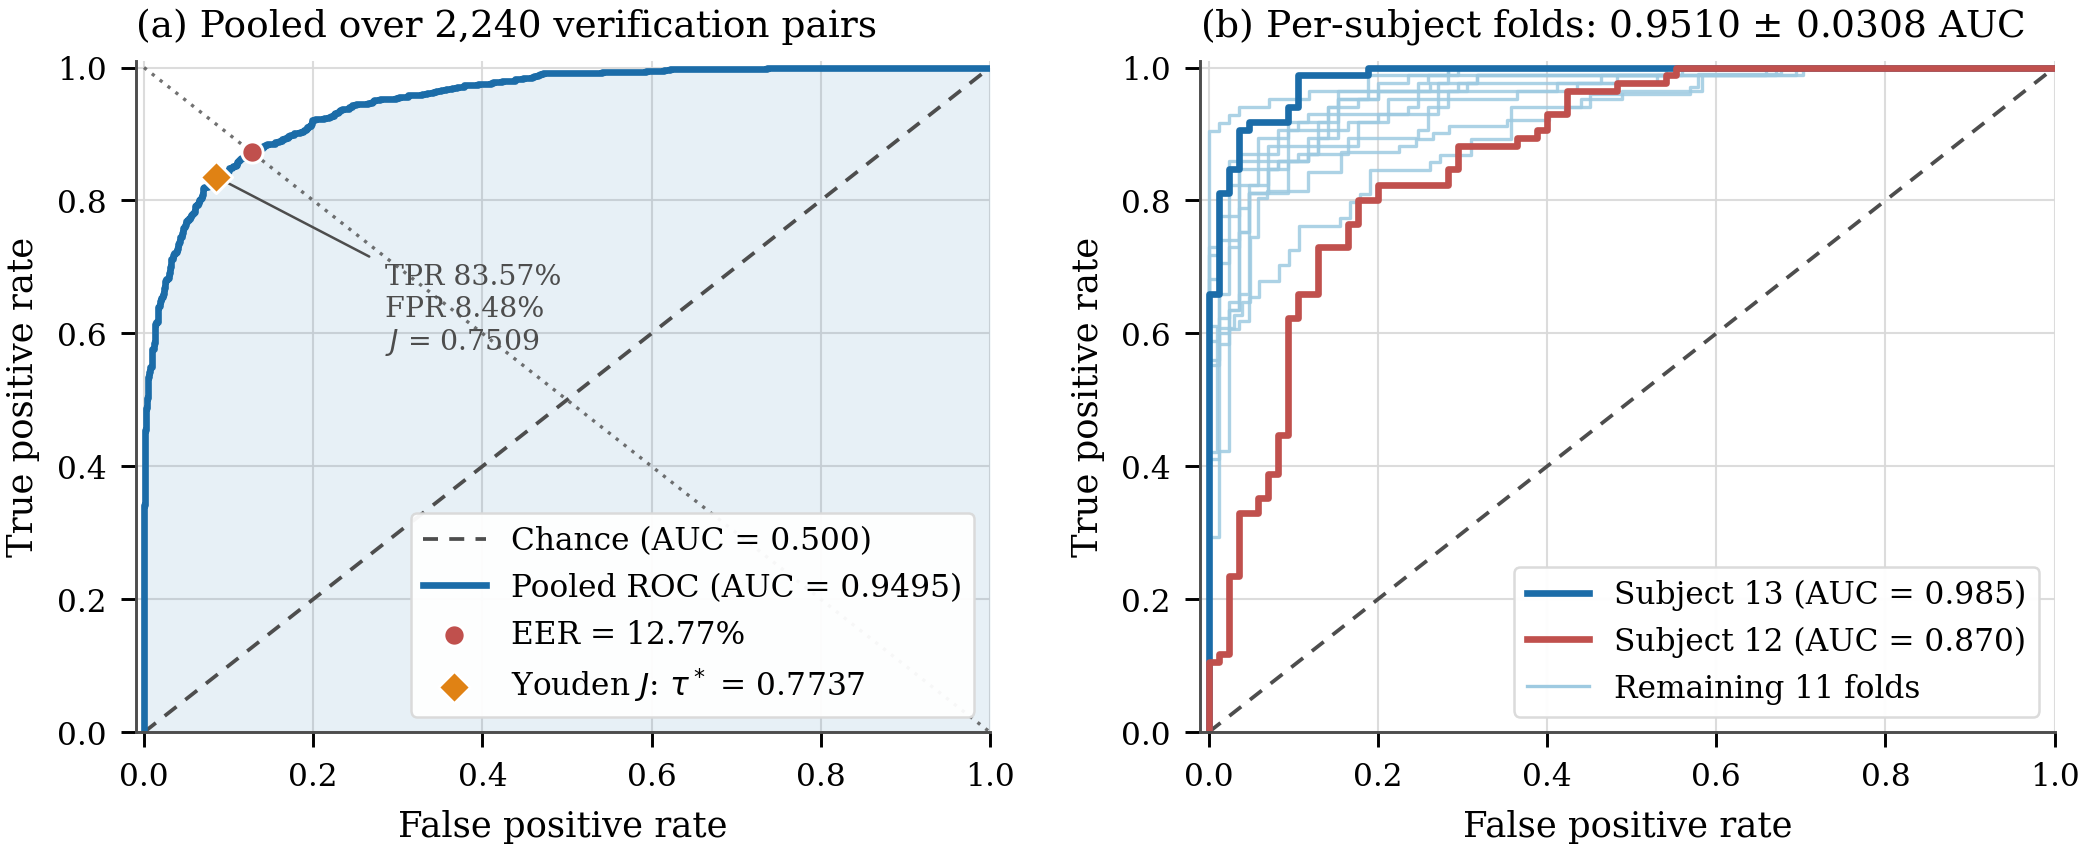
\includegraphics[width=\textwidth]{../figures/fig5_roc.png}
\caption{ROC analysis of the leave-one-subject-out evaluation. (a) Pooled over
all 2{,}240 verification pairs, with the equal-error point and the
Youden-optimal operating point $\tau^* = 0.7737$ marked; the two sit far apart,
which is why the operating point must be reported alongside the AUC rather than
assumed. (b) All 13 subject-held-out folds overlaid, with the best (Subject 13,
$0.985$) and worst (Subject 12, $0.870$) drawn in full. The envelope is narrow
through the mid-range and widens near the origin, indicating that
low-false-accept operation is the regime where subject identity matters most.}
\label{fig:roc}
\end{figure*}

\subsection{Per-Fold Dispersion}
\label{sec:perfold}

Table~\ref{tab:perfold} and Fig.~\ref{fig:spread} give the fold-level detail
that an aggregate $\pm\sigma$ suppresses. The distribution is unimodal with a
single clear low outlier: Subject 12 yields $87.00\%$ AUC and $77.65\%$
accuracy, roughly $2.6$ standard deviations below the mean accuracy, while the
remaining twelve folds fall between $82.14\%$ and $92.35\%$. Removing that fold
would raise mean accuracy to $87.83\%$; we report it included.

Two structural observations follow. First, the ordering of folds is stable
across metrics---the subjects that are hard by AUC are hard by accuracy, F1 and
EER alike---which points to a property of those subjects' gait rather than to
threshold artefacts. Second, precision and recall trade off across folds in
opposite directions (Subject 6: $95.59\%$ precision, $76.47\%$ recall; Subject 9:
$81.00\%$ precision, $95.29\%$ recall), meaning a single global threshold sits
at a different point on each subject's curve. Per-subject calibration is a
natural extension we did not pursue.

\begin{table}[!t]
\caption{Per-Fold LOOCV Results (Held-Out Subject; \%)}
\label{tab:perfold}
\centering
\small
\begin{tabular}{@{}lrrrrrrr@{}}
\toprule
\tabhead{Subj.} & \tabhead{Acc} & \tabhead{F1} & \tabhead{Prec} &
\tabhead{Rec} & \tabhead{AUC} & \tabhead{EER} & \tabhead{$n$} \\
\midrule
S1  & 89.29 & 90.00 & 84.38 & 96.43 & 98.16 &  6.55 & 168 \\
S2  & 87.65 & 87.72 & 87.21 & 88.24 & 95.04 & 12.94 & 170 \\
S3  & 88.24 & 88.10 & 89.16 & 87.06 & 95.54 & 11.76 & 170 \\
S4  & 82.14 & 81.01 & 86.49 & 76.19 & 90.87 & 19.05 & 168 \\
S5  & 84.80 & 84.26 & 87.37 & 81.37 & 92.59 & 15.69 & 204 \\
S6  & 86.47 & 84.97 & 95.59 & 76.47 & 96.71 &  9.41 & 170 \\
S7  & 88.24 & 88.76 & 84.95 & 92.94 & 95.70 &  9.41 & 170 \\
S8  & 88.24 & 88.64 & 85.71 & 91.76 & 96.64 & 12.94 & 170 \\
S9  & 86.47 & 87.57 & 81.00 & 95.29 & 95.71 & 11.76 & 170 \\
S10 & 90.00 & 89.94 & 90.48 & 89.41 & 97.20 &  9.41 & 170 \\
S11 & 90.00 & 90.50 & 86.17 & 95.29 & 96.62 & 11.76 & 170 \\
S12 & 77.65 & 78.65 & 75.27 & 82.35 & 87.00 & 20.00 & 170 \\
S13 & 92.35 & 92.49 & 90.91 & 94.12 & 98.53 &  8.82 & 170 \\
\midrule
Mean    & 87.04 & 87.12 & 86.51 & 88.23 & 95.10 & 12.27 & \\
Std     &  3.65 &  3.77 &  4.72 &  6.82 &  3.08 &  3.80 & \\
\bottomrule
\end{tabular}
\end{table}

\begin{figure*}[!t]
\centering
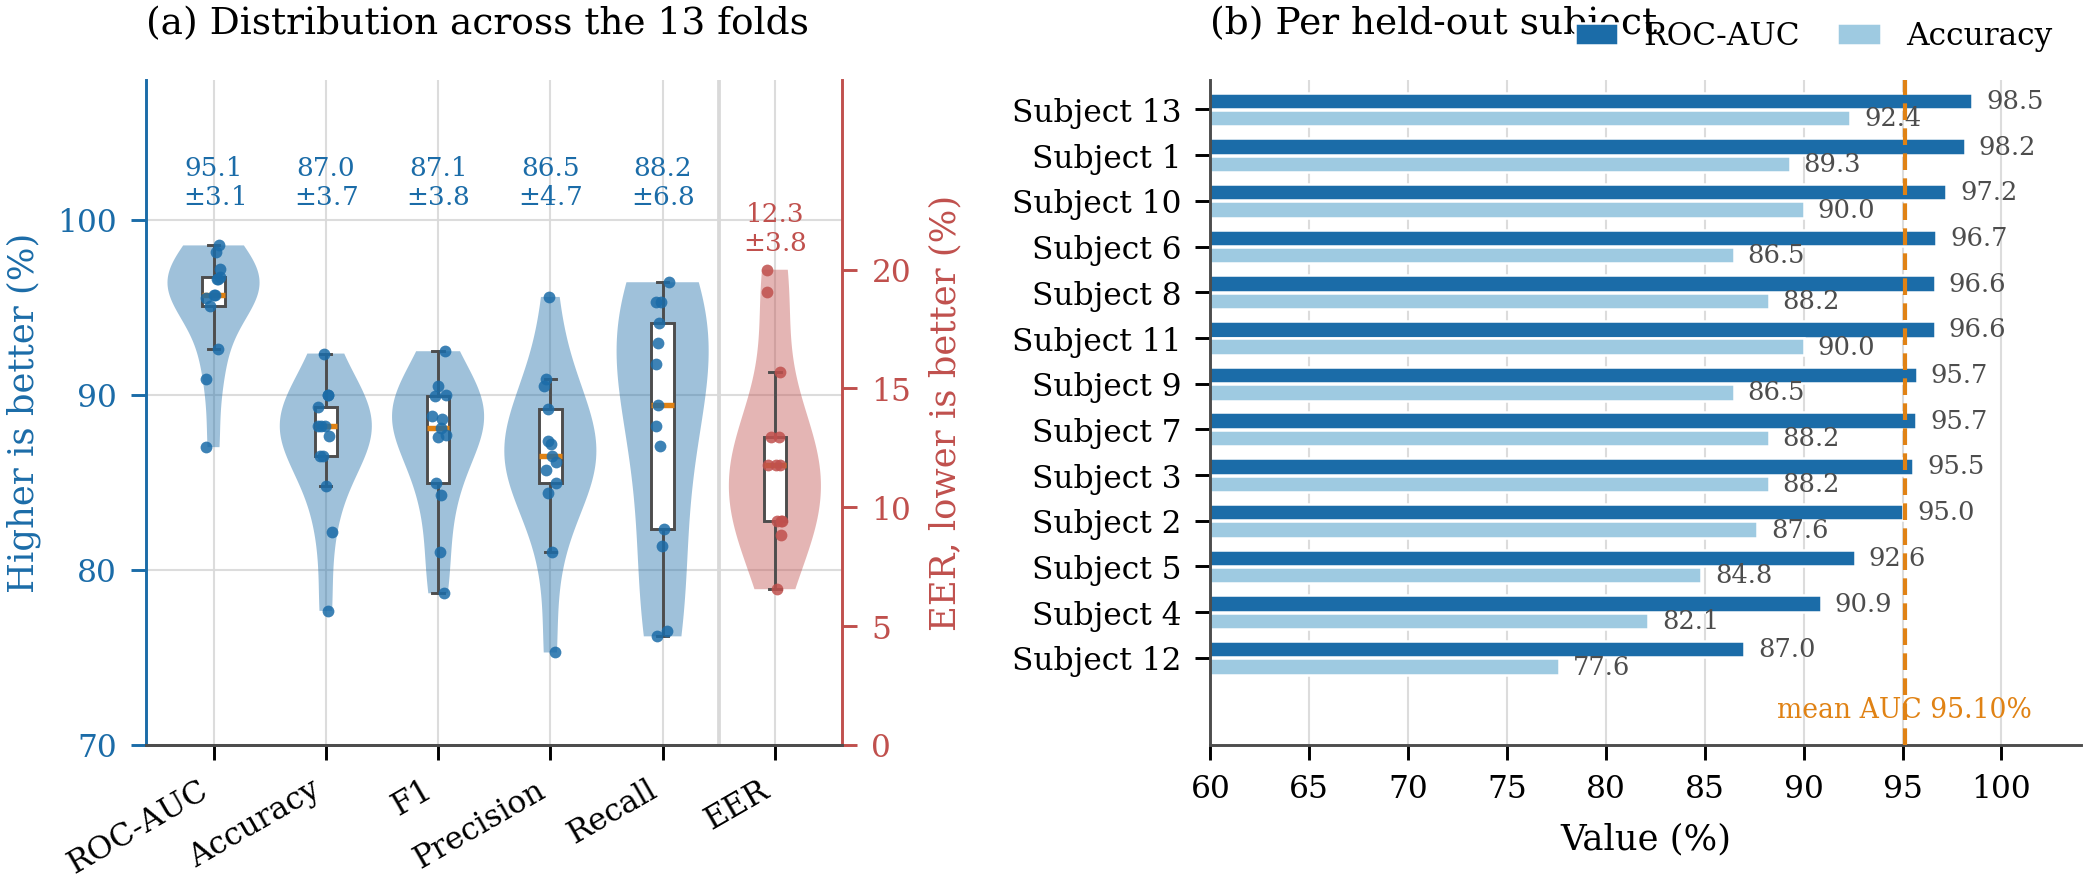
\includegraphics[width=\textwidth]{../figures/fig8_loocv_spread.png}
\caption{Fold-to-fold dispersion across the 13 subject-held-out folds. (a)
Distribution of each metric, with individual folds overplotted; EER is drawn
against its own right-hand scale because its $6.6$--$20.0\%$ range would
otherwise compress the remaining five into an unreadable band. The
distributions are unimodal, confirming that the reported $\pm\sigma$ summarises
a coherent spread rather than concealing a split population. (b) Per-subject
ROC-AUC and accuracy, ordered by AUC. One fold (Subject 12) sits clearly below the
rest on every metric; the remaining twelve span roughly ten accuracy points.}
\label{fig:spread}
\end{figure*}

\subsection{Operating Points and Error Structure}

Fig.~\ref{fig:confusion} contrasts the two operating points, and the
difference between them matters for deployment. At the native $\tau = 0.5$ the
system produces 987 true positives, 962 true negatives, 158 false positives and
133 false negatives---balanced errors, $87.01\%$ accuracy. Moving to the
Youden-optimal $\tau^* = 0.7737$ shifts 63 pairs from false-positive to
true-negative at the cost of 51 additional false negatives: false positives
fall from 158 to 95 and precision rises from $86.20\%$ to $90.79\%$, while
recall falls from $88.12\%$ to $83.57\%$.

Which of these is preferable is a policy question, not a modelling one. In a
forensic screening context a false positive means accepting a forgery, and the
stricter threshold is the right default. We flag one inconsistency in earlier
descriptions of this system for the record: the frequently quoted
$987/962/158/133$ confusion matrix is the $\tau = 0.5$ matrix, not the
Youden-threshold matrix, though it has sometimes been reported alongside
$\tau^* = 0.7737$.

\begin{figure*}[!t]
\centering
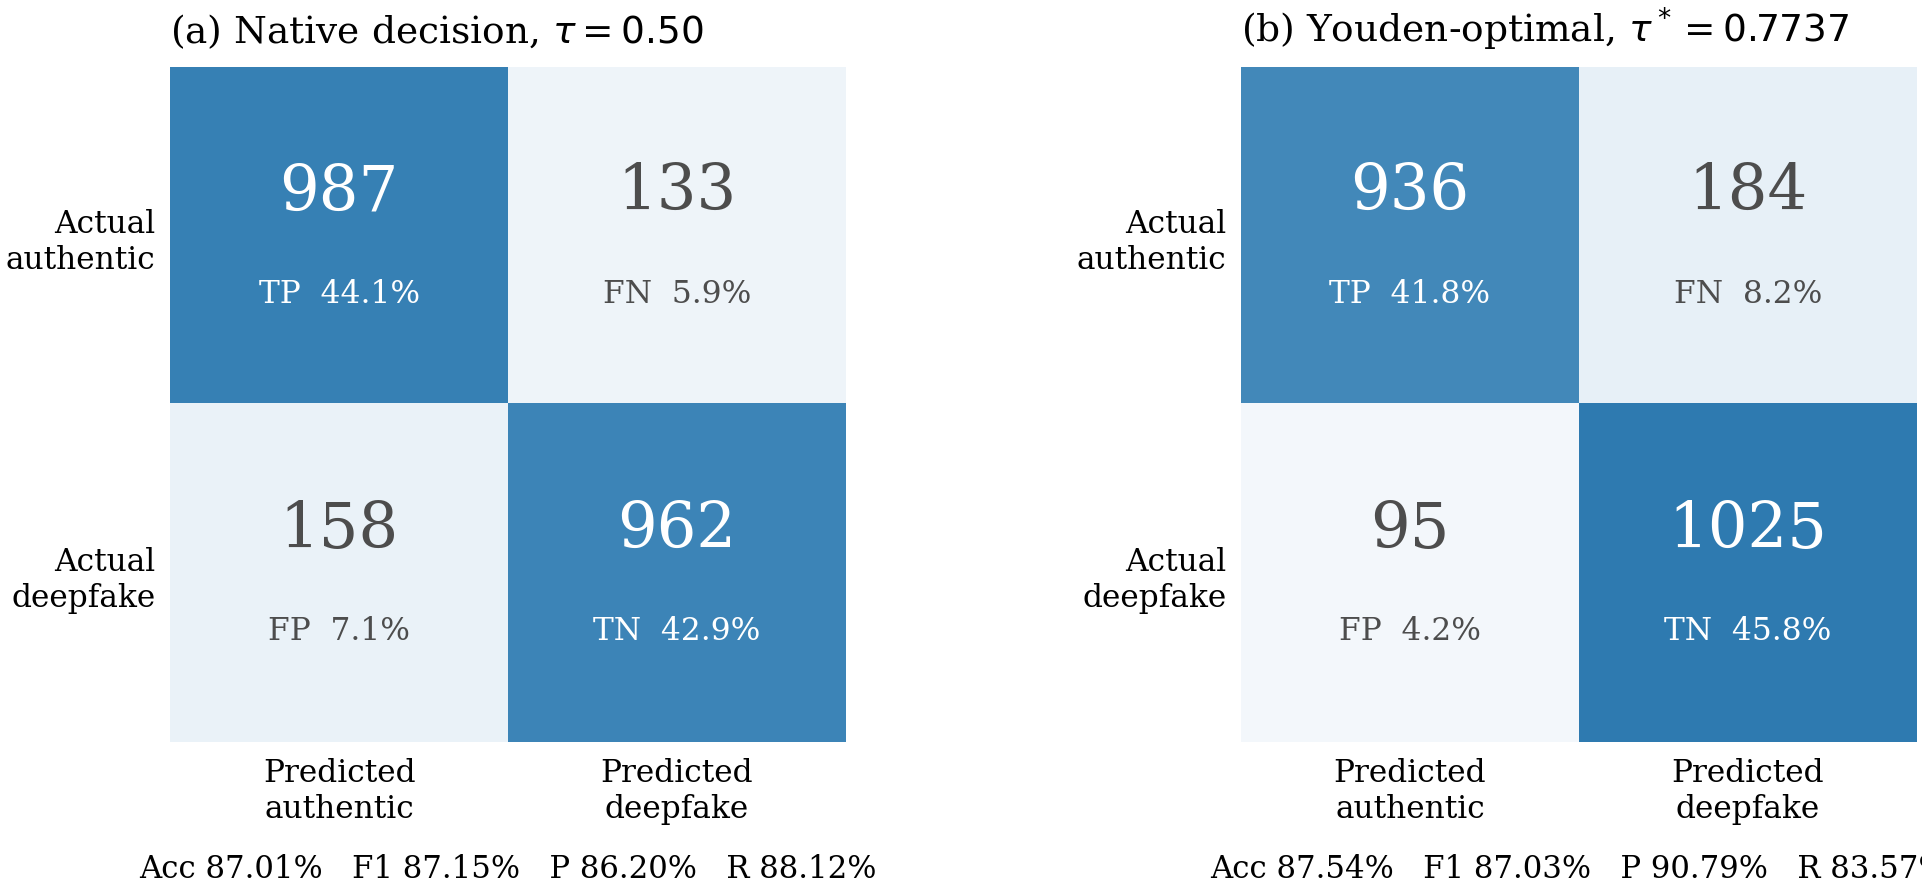
\includegraphics[width=\textwidth]{../figures/fig6_confusion.png}
\caption{Pooled confusion matrices over all 2{,}240 LOOCV verification pairs at
the two operating points. (a) The network's native $\tau = 0.5$ argmax
decision, which is the point at which the per-fold metrics of
Table~\ref{tab:perfold} were computed. (b) The Youden-optimal $\tau^* = 0.7737$
actually applied at inference. Tightening the threshold converts 63 false
accepts into correct rejections at the cost of 51 additional false rejections,
raising precision from $86.20\%$ to $90.79\%$ while lowering recall from
$88.12\%$ to $83.57\%$. The two matrices should not be quoted interchangeably.}
\label{fig:confusion}
\end{figure*}

The score distribution in Fig.~\ref{fig:score} explains why the two thresholds
differ so much while yielding similar accuracy. Both classes are strongly
saturated---genuine pairs have median score $0.999$, impostor pairs $0.0007$---%
so the region between the two thresholds contains only 86 pairs, $3.8\%$ of the
total. The classifier is confident almost everywhere and the threshold choice
redistributes a small, hard residue.

\begin{figure}[!t]
\centering
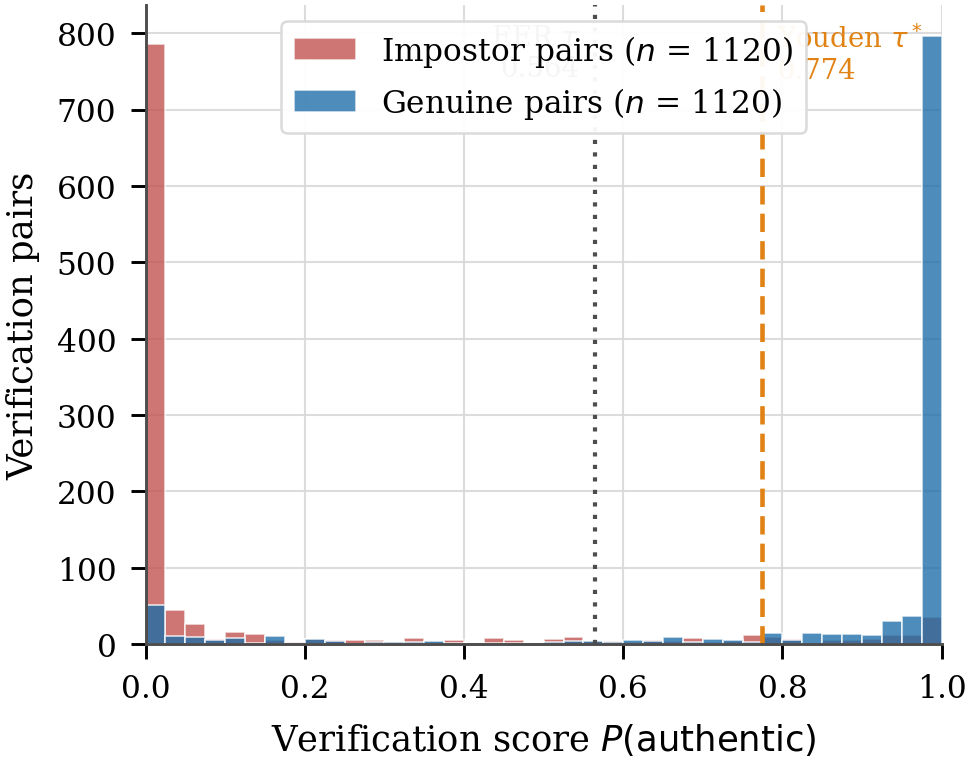
\includegraphics[width=\columnwidth]{../figures/fig7_score_distribution.png}
\caption{Distribution of $P(\textsc{authentic})$ over the 2{,}240 pooled
verification pairs. Both classes saturate against their extremes (genuine
median $0.999$, impostor median $0.0007$), leaving only 86 pairs---$3.8\%$ of
the total---between the equal-error and Youden thresholds. The model is
decisive on the large majority of pairs, and threshold selection governs the
disposition of a small ambiguous residue rather than shifting bulk behaviour.
The corollary is that reported confidence values should not be read as
calibrated probabilities.}
\label{fig:score}
\end{figure}

\subsection{Architectural Ablation}
\label{sec:ablation-results}

The dual-path stack of Section~\ref{sec:aux} is inert in the deployed
checkpoint. The obvious question is whether it should be: would wiring it onto
the decision path improve verification? Table~\ref{tab:ablation} and
Fig.~\ref{fig:ablation} answer it.

We construct five variants that differ only in how the observed and claimed
sequences are encoded before they are compared. Each encodes both sequences
with shared weights, preserves the time axis, and forms the same per-timestep
comparison tensor, which the same temporal CNN and classifier then consume. The
control, \emph{Raw}, uses an identity encoder and therefore reproduces the
deployed model exactly at $133{,}058$ parameters. Four \emph{Raw~+~X} variants
concatenate the encoded comparison onto the raw one, so each contains the
deployed model's evidence and can only justify itself by improving on it.
\emph{Hybrid only} removes the raw comparison, isolating what the encoder
contributes alone. Every variant is trained under the full leave-one-subject-out
protocol at three random seeds, giving $13 \times 3 = 39$ observations per
variant on identical folds and identical initialisations.

The result is unambiguous and it is negative. The deployed model is the best of
the five, at $94.25\% \pm 3.09\%$ ROC-AUC. Every encoder variant is worse, and
because all variants share folds and seeds the comparison can be made pairwise,
which removes fold difficulty and initialisation luck. The paired deficits
range from $-2.53$ points for \emph{Raw~+~CNN} to $-5.93$ for
\emph{Raw~+~BiLSTM}; all four are significant at $p < 10^{-3}$
(two-sided paired $t$-test, $n = 39$), and no variant wins more than 9 of its
39 paired trials. The $95\%$ confidence interval on each deficit lies wholly
below zero (Fig.~\ref{fig:ablation}b). Adding capacity does not merely fail to
help: the largest variant, at $981{,}000$ parameters, is $4.22$ points worse
than the $133{,}058$-parameter control.

\emph{Hybrid only} settles which half of the architecture carries the signal.
Stripped of the raw per-timestep comparison, it reaches $50.70\% \pm 20.81\%$
ROC-AUC---indistinguishable from chance, and with a standard deviation four
times that of any other variant, indicating it often fails to learn at all. The
discriminative information is in the direct per-dimension comparison between
the observed sequence and the enrolled signature, where dimension $j$ of each is
the same physical quantity and subtraction is meaningful. Passing both through
a learned encoder first destroys that correspondence and forces the classifier
to recover it from a representation that begins as a random projection.

Two consequences follow. First, the ablation retroactively justifies the
deployed architecture: the inert branch of Section~\ref{sec:aux} is not a
missed opportunity, and connecting it would cost accuracy. Second, the result
is a caution against the assumption that a richer temporal encoder is a free
improvement. On this task, with this cohort size, it is a reliable
regression.

\begin{table}[!t]
\caption{LOOCV Ablation Over 13 Folds and 3 Seeds ($n = 39$ Paired
Observations per Variant). $\Delta$ is the Paired Change in ROC-AUC Against the
Deployed Model}
\label{tab:ablation}
\centering
\footnotesize
\begin{tabular}{@{}lrrrr@{}}
\toprule
\tabhead{Variant} & \tabhead{Params} & \tabhead{ROC-AUC (\%)} &
\tabhead{Acc (\%)} & \tabhead{$\Delta$ AUC} \\
\midrule
Raw (deployed)     & 133{,}058 & $\mathbf{94.25 \pm 3.09}$ & $\mathbf{86.04}$ & --- \\
Raw + CNN          & 434{,}690 & $91.72 \pm 4.13$ & $82.66$ & $-2.53^{\ast}$ \\
Raw + Transformer  & 712{,}002 & $90.37 \pm 5.13$ & $80.32$ & $-3.88^{\ast}$ \\
Raw + Hybrid       & 980{,}994 & $90.03 \pm 6.11$ & $81.26$ & $-4.22^{\ast}$ \\
Raw + BiLSTM       & 379{,}074 & $88.32 \pm 6.08$ & $74.84$ & $-5.93^{\ast}$ \\
Hybrid only        & 876{,}162 & $50.70 \pm 20.81$ & $49.37$ & $-43.55^{\ast}$ \\
\bottomrule
\end{tabular}

\vspace{2pt}
\raggedright\footnotesize
$^{\ast}$Significant at $p < 10^{-3}$, two-sided paired $t$-test over the 39
matched (fold, seed) pairs. ``Hybrid only'' omits the raw comparison entirely.
\end{table}

\begin{figure*}[!t]
\centering
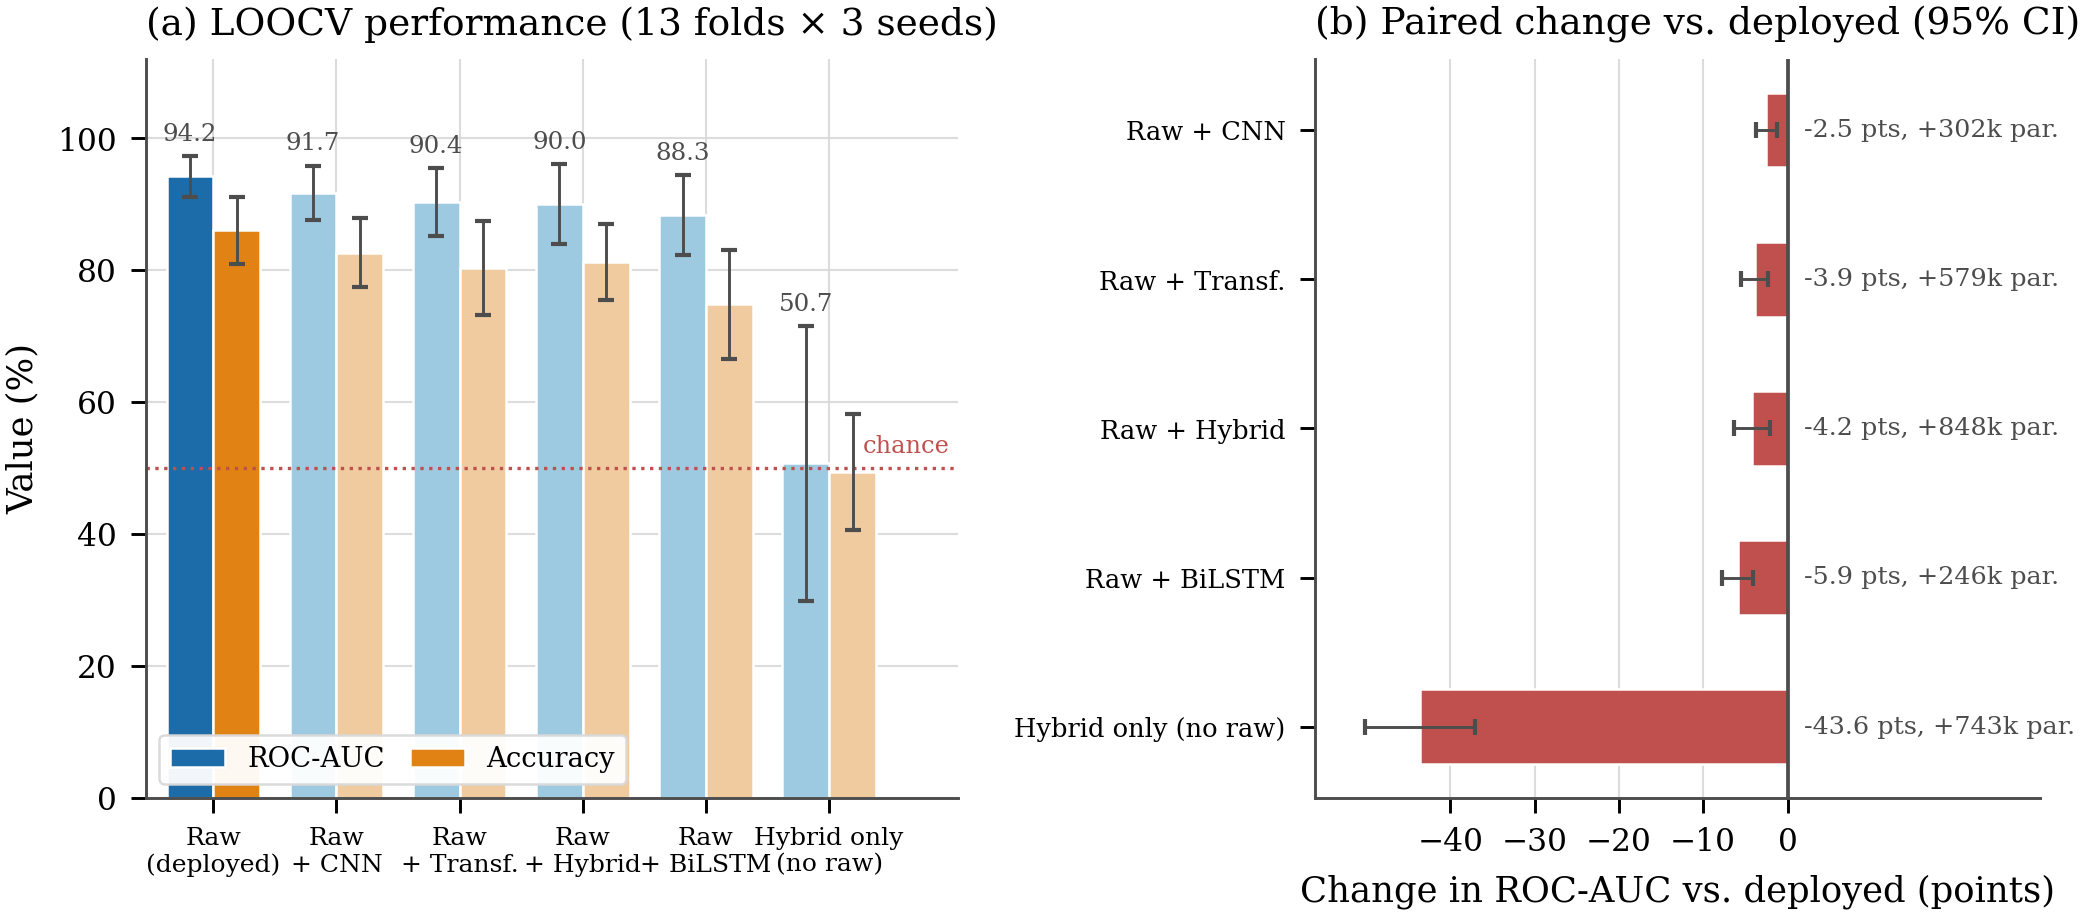
\includegraphics[width=\textwidth]{../figures/fig9_ablation.png}
\caption{LOOCV ablation over five variants, each measured on 13
subject-held-out folds at 3 seeds. (a) ROC-AUC and accuracy per variant, with
standard deviation across the 39 observations; the deployed model (dark) is
best, and removing the raw per-timestep comparison entirely (rightmost) lands
at chance. (b) Because every variant shares folds and seeds with the control,
the comparison is made pairwise, removing fold difficulty and initialisation
luck. All five $95\%$ confidence intervals lie wholly below zero. The deficit
does not shrink as parameters are added: the largest variant is $4.22$ points
worse than a control one-seventh its size.}
\label{fig:ablation}
\end{figure*}

\subsection{Face-Swap Video Validation}
\label{sec:deepfake-results}

Three face-swapped clips were generated as described in
Section~\ref{sec:setup}, pairing enrolled subjects so that both the body source
and the face source have enrolled signatures. The mechanism the protocol tests
is not in question: an InSwapper-class pipeline composites through a mask
confined to the facial region, leaving the skeletal trajectory of the body
subject intact by construction, so the gait recovered from a forged clip is the
body subject's. Each clip was scored against the claimed (face) identity using
checkpoint\_epoch\_46\_best.pth at the LOOCV Youden threshold
$\tau^* = 0.7737$, and independently re-scored against every enrolled identity
to identify the closest match.

All three clips were correctly rejected. Table~\ref{tab:deepfake-video} reports
the similarity to the claimed identity, the identity the system actually
matched, and the similarity to that match. In every case the claimed identity
scores below $0.006$---four to six orders of magnitude below
$\tau^*$---while the true body source scores above $0.9998$. The system does
not merely fail to confirm the claimed identity; it confidently identifies the
correct one, exactly as the threat model of Section~\ref{sec:threat} predicts.
Frame extraction succeeded on the full length of all three clips (135, 149 and
327 valid frames respectively), so the result is not an artefact of partial
pose failure on manipulated footage.

One result merits a caveat rather than a footnote. For
Subject~8\_body\_Subject~5\_face, the correct match (Subject~8, $0.99999$) is
nearly tied by an impostor score for Subject~10 ($0.99986$)---the two
nearest scores in the entire validation, four orders of magnitude closer than
any other pair in Table~\ref{tab:deepfake-video}. The system still ranks the
true body source first and still rejects the claimed identity by a wide margin,
so the clip is correctly handled; but the near-collision shows that the
embedding space is not uniformly well separated across all subject pairs, and
a larger validation set would be needed to establish how often this occurs.

\begin{table}[!t]
\caption{Face-Swap Video Validation ($n=3$; Existence Check, Not a
Statistically Powered Result)}
\label{tab:deepfake-video}
\centering
\small
\begin{tabular}{@{}lcccc@{}}
\toprule
\tabhead{Clip (body\_face)} & \tabhead{Claimed} & \tabhead{Sim.} &
\tabhead{Matched} & \tabhead{Sim.} \\
\midrule
Subj.6\_Subj.3 & Subj.\,3 & 0.0057 & Subj.\,6 & 0.9999 \\
Subj.7\_Subj.11 & Subj.\,11 & 0.0003 & Subj.\,7 & 0.9999 \\
Subj.8\_Subj.5  & Subj.\,5 & $<$0.0001 & Subj.\,8 & 0.99999$^{\ast}$ \\
\bottomrule
\end{tabular}

\vspace{2pt}
\raggedright\footnotesize
$^{\ast}$Nearest impostor score for this clip (Subject~10) was $0.99986$,
the closest margin observed; see discussion in text.
\end{table}

We report the scope of this result precisely rather than overstate it. Three
clips, drawn from a single face-swap pipeline (FaceFusion / InSwapper) under
one masking configuration, is an existence check confirming the mechanism
behaves as the threat model predicts---it is not a statistically powered
validation, and it says nothing about behaviour under other face-swap models,
face-enhancement post-processing, or heavier recompression.
Section~\ref{sec:threats} states what a properly powered version of this
experiment would require.

% ===========================================================================
\section{Explainability}
\label{sec:explain}

\subsection{Attribution Method}

To determine what the verification network uses, we compute gradient-times-input
attribution on the 78-dimensional descriptor. For a sample scored towards class
$c$, we backpropagate the corresponding logit to the input and take
\begin{equation}
A_{t,j} = \left| \hat{f}_{t,j} \cdot
\frac{\partial \ell_c}{\partial \hat{f}_{t,j}} \right|,
\end{equation}
aggregating over timesteps and over the three coordinates belonging to each
joint, then normalising to $[0,1]$. We additionally compute
Grad-CAM~\cite{gradcam} over the final convolutional layer for temporal
localisation. Attribution is averaged over 26 samples, two per identity.

Because the gradient path runs through the verification head, this attribution
describes the function that actually produces the verdict. We use the term
gradient-times-input rather than Grad-CAM for the joint analysis, since the
former is what the joint-level numbers are computed
with~\cite{shrikumar,sundararajan}.

\subsection{Joint-Level Attribution}

Fig.~\ref{fig:joints} and Table~\ref{tab:joints} give the ranking. The left
shoulder receives the highest attribution ($1.000$), followed by the right heel
($0.940$), left foot index ($0.931$) and left knee ($0.897$); both hips rank
lowest (left $0.665$, right $0.566$).

The structure is biomechanically coherent. The two extremes of the kinematic
chain dominate: shoulders, which carry the trunk countermotion that balances
angular momentum during swing, and the distal foot segments, which register
heel strike and toe-off---the discrete, individually-variable events that
define the gait cycle~\cite{perry_gait,winter_biomech}. The hips rank lowest,
which is expected rather than anomalous: the pelvis centre is the origin of the
coordinate normalisation, so hip positions are near-constant by construction
and carry little residual variance.

A left--right asymmetry is visible (left shoulder $1.000$ against right
$0.873$; left foot $0.931$ against right $0.766$; but right heel $0.940$
against left $0.709$). We do not over-interpret it. With 13 subjects and 26
attribution samples it is as consistent with cohort-specific gait asymmetry, or
with viewpoint bias between the frontal and side recordings, as with anything
the model has learned about laterality in general.

\begin{figure*}[!t]
\centering
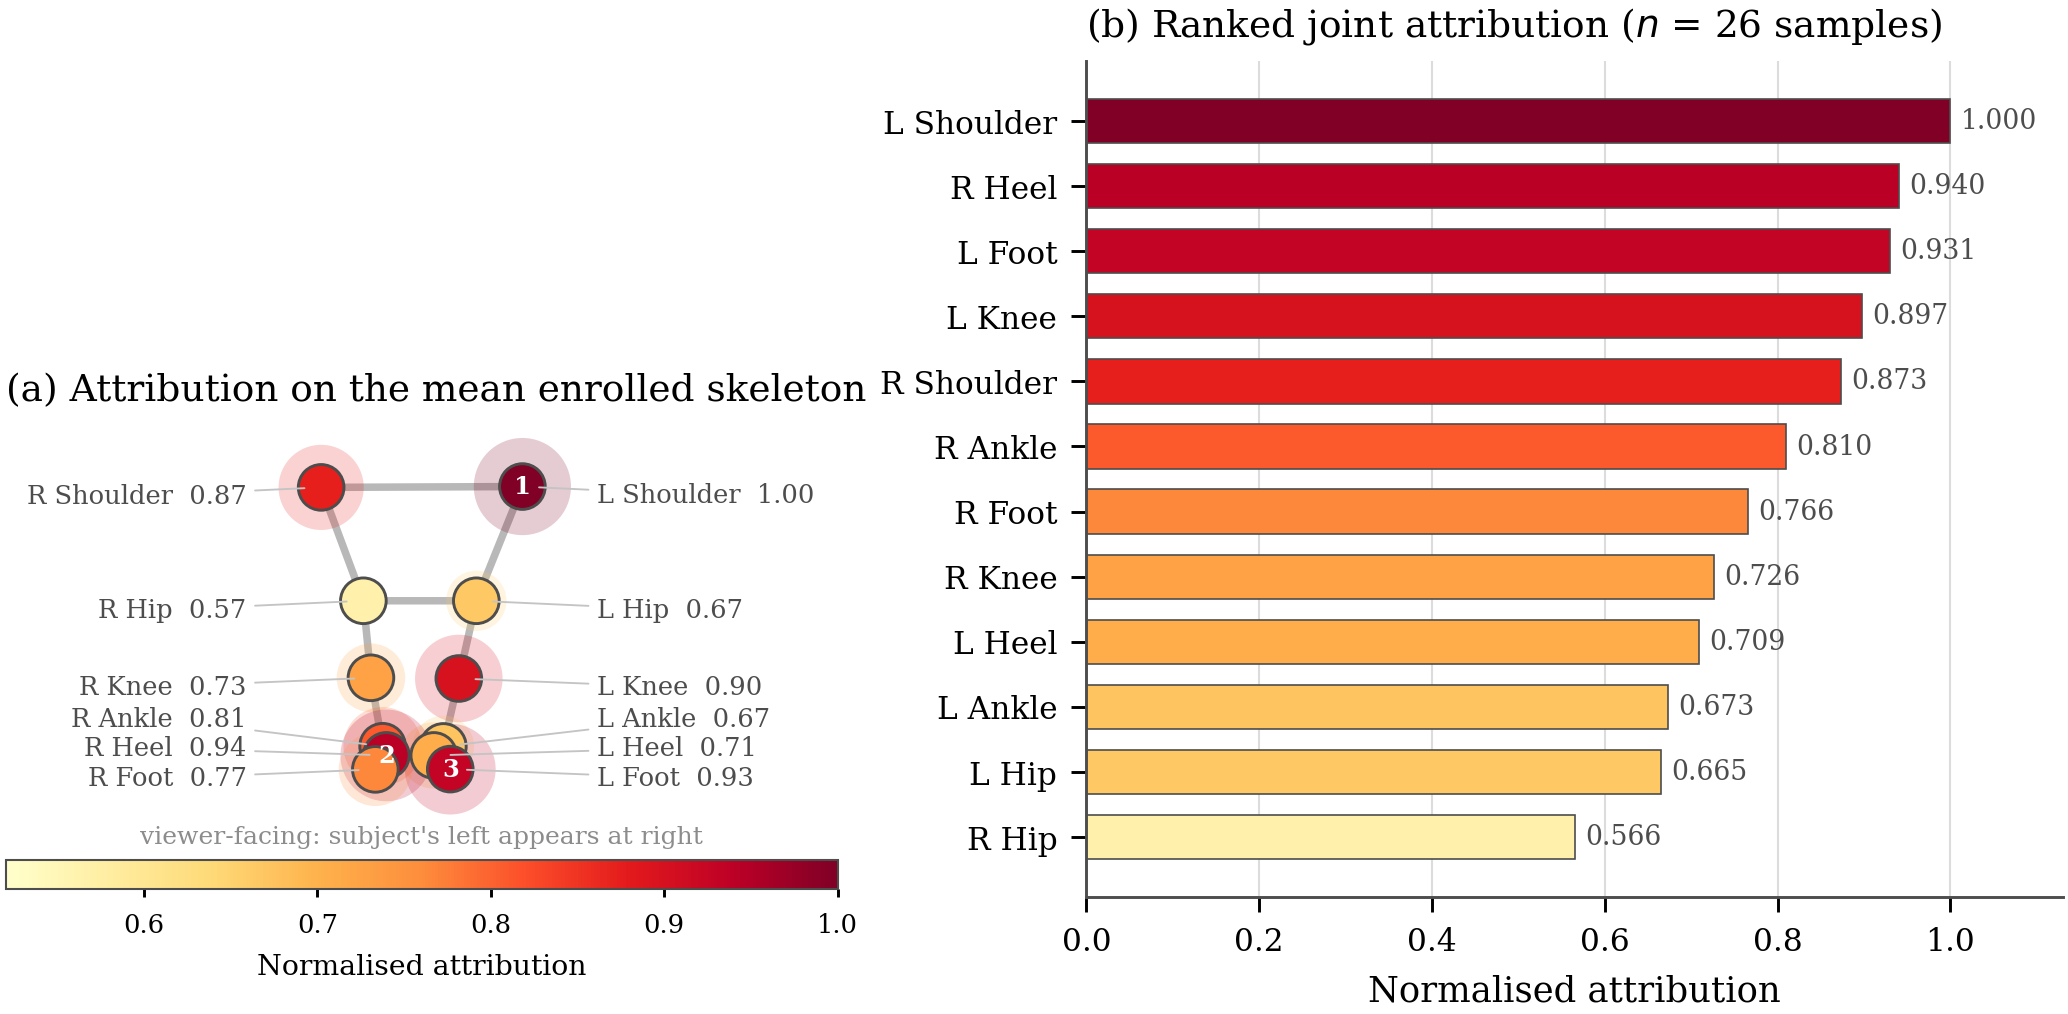
\includegraphics[width=\textwidth]{../figures/fig10_joint_importance.png}
\caption{Gradient-times-input attribution over the 12 gait keypoints, averaged
across 26 samples (two per identity). (a) Attribution rendered on a skeleton
whose geometry is the mean of all 13 enrolment signatures across their 60
timesteps, so the layout is data-derived; marker size and colour both encode
attribution. (b) The same values ranked. Attribution concentrates at the two
ends of the kinematic chain---shoulder countermotion and distal heel-strike and
toe-off structure---while the hips rank lowest, as expected given that the
pelvis centre is the origin of the coordinate normalisation and therefore
carries little residual variance.}
\label{fig:joints}
\end{figure*}

\begin{table}[!t]
\caption{Joint Attribution Ranking (Normalised, 26 Samples)}
\label{tab:joints}
\centering
\footnotesize
\begin{tabular}{@{}clc@{\hskip 8pt}clc@{}}
\toprule
\tabhead{Rank} & \tabhead{Joint} & \tabhead{Score} &
\tabhead{Rank} & \tabhead{Joint} & \tabhead{Score} \\
\midrule
1 & Left shoulder   & 1.000 & 7  & Right foot index & 0.766 \\
2 & Right heel      & 0.940 & 8  & Right knee       & 0.726 \\
3 & Left foot index & 0.931 & 9  & Left heel        & 0.709 \\
4 & Left knee       & 0.897 & 10 & Left ankle       & 0.673 \\
5 & Right shoulder  & 0.873 & 11 & Left hip         & 0.665 \\
6 & Right ankle     & 0.810 & 12 & Right hip        & 0.566 \\
\bottomrule
\end{tabular}
\end{table}

\subsection{Feature-Group Attribution}

Table~\ref{tab:groups} and Fig.~\ref{fig:groups} decompose attribution by
feature block. Coordinates take $47.68\%$, velocities $37.40\%$ and joint
angles $14.92\%$. Read as raw shares this simply says that coordinates matter
most, which is unsurprising given that they occupy 36 of 78 dimensions.

The informative comparison is against dimensional share. Coordinates and
velocities each occupy $46.15\%$ of the input and draw $47.68\%$ and $37.40\%$
of attribution respectively---ratios of $1.03$ and $0.81$. Joint angles occupy
$7.69\%$ of the input and draw $14.92\%$: a ratio of $1.94$. Per dimension, the
six angle features are roughly twice as influential as the average coordinate
and nearly two and a half times as influential as the average velocity.

This is the clearest practical finding in the attribution analysis. The six
scale-free, rotation-invariant biomechanical constraints are the most
information-dense part of the descriptor, which suggests that a
cheaper feature set weighted towards angular kinematics may retain most of the
discriminative power---directly relevant to the embedded deployment discussed
in Section~\ref{sec:discussion}. Within the angle block
(Fig.~\ref{fig:groups}b), the left ankle ($1.000$) and left knee ($0.896$)
dominate, consistent with the distal emphasis in the joint-level ranking.

\begin{table}[!t]
\caption{Attribution by Feature Group, Against Dimensional Share}
\label{tab:groups}
\centering
\small
\begin{tabular}{@{}lccccc@{}}
\toprule
\tabhead{Group} & \tabhead{Attrib.} & \tabhead{Dims} &
\tabhead{Dim.} & \tabhead{Ratio} \\
 & \tabhead{(\%)} & & \tabhead{share (\%)} & \\
\midrule
Normalised coordinates & 47.68 & 36 & 46.15 & 1.03 \\
Velocities             & 37.40 & 36 & 46.15 & 0.81 \\
Joint angles           & 14.92 &  6 &  7.69 & \textbf{1.94} \\
\bottomrule
\end{tabular}
\end{table}

\begin{figure*}[!t]
\centering
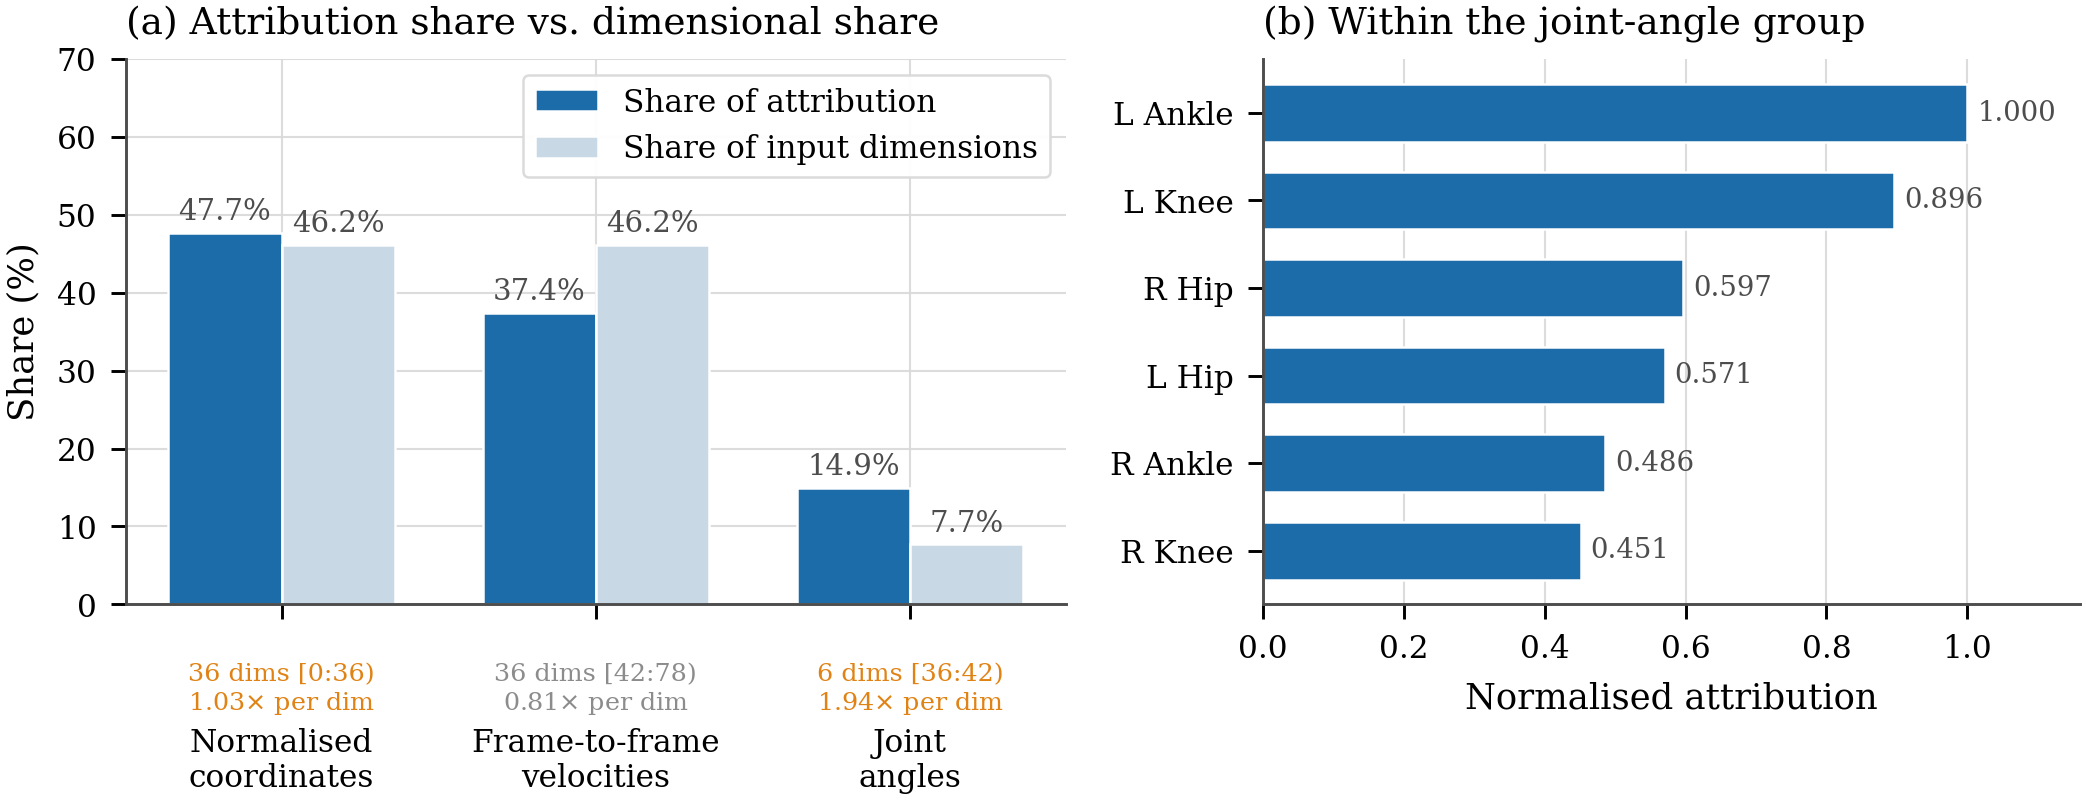
\includegraphics[width=\textwidth]{../figures/fig11_feature_groups.png}
\caption{Attribution by feature group. (a) Each group's share of total
attribution against its share of the 78 input dimensions. Coordinates and
velocities draw roughly their proportional share ($1.03\times$ and
$0.81\times$ per dimension), whereas the six joint angles draw $1.94\times$
theirs---per dimension they are the most information-dense part of the
descriptor, despite being the smallest block. (b) Within the angle block, the
left ankle and left knee dominate, echoing the distal emphasis seen in the
joint-level ranking.}
\label{fig:groups}
\end{figure*}

% ===========================================================================
\section{Discussion}
\label{sec:discussion}

\subsection{Comparative Positioning}

Table~\ref{tab:comparison} situates this work against the literature of
Section~\ref{sec:related}. We stress that the table is not a ranking. Every row
is measured on a different corpus under a different protocol against a
different task, and our own figure is a leave-one-subject-out result on a
13-subject corpus collected by the authors---a fundamentally different
quantity from a cross-dataset AUC on Celeb-DF. Reading our $94.95\%$ as
exceeding AltFreezing's $89.5\%$ would be a category error, and we do not make
that claim. The table's purpose is to show where the modality and task sit
relative to established work.

\begin{table*}[!t]
\caption{Positioning Against Related Work. Figures Are Not Directly
Comparable: Each Row Reports a Different Task, Corpus and Protocol}
\label{tab:comparison}
\centering
\small
\begin{tabular}{@{}llllll@{}}
\toprule
\tabhead{Method} & \tabhead{Venue} & \tabhead{Task} & \tabhead{Modality} &
\tabhead{Reported figure} & \tabhead{Corpus / protocol} \\
\midrule
Agarwal \emph{et al.}~\cite{agarwal2019} & CVPRW 2019 & Deepfake det.
  & Facial + head motion & --- & Per-individual profiles \\
FTCN~\cite{ftcn} & ICCV 2021 & Face forgery det.
  & Face RGB & $\sim$86--89\% AUC & Celeb-DF, cross-dataset \\
RECCE~\cite{recce} & CVPR 2022 & Face forgery det.
  & Face RGB & $\sim$70.9\% AUC & Celeb-DF-v2, cross-dataset \\
GaitFormer~\cite{gaitformer} & Sensors 2022 & Gait recognition
  & Skeleton & 92.5\% acc. & CASIA-B \\
AltFreezing~\cite{altfreezing} & CVPR 2023 & Face forgery det.
  & Face RGB & 89.5\% AUC & Celeb-DF, cross-dataset \\
GaitPT~\cite{gaitpt} & IEEE FG 2024 & Gait recognition
  & Skeleton & 82.6\% acc. & CASIA-B \\
Petmezas \emph{et al.}~\cite{hybrid_face} & MTA 2024 & Identity verification
  & Face + 3DMM & --- & VoxCeleb2 \\
TT-DF~\cite{ttdf} & Preprint 2025 & Body forgery det.
  & Pose / motion & --- & TT-DF benchmark \\
\midrule
\textbf{This work} & --- & \textbf{Face-swap det.}
  & \textbf{Skeleton gait} & \textbf{94.95\% AUC}
  & \textbf{GaitDeepfake-13, LOOCV} \\
\bottomrule
\end{tabular}
\end{table*}

Gait evidence has also begun to appear in forensic practice: a commercial gait
and body-structure analysis was reported in 2025 to have been accepted as
evidence in a European murder case where the subject's face occupied roughly
$10 \times 5$ pixels~\cite{forensic_gait}. We cite this as an industry
milestone and note its limits precisely---it is a single trade-press account of
a forensic report admitted in a case not yet tried, not an appellate ruling or
a peer-reviewed forensic validation, and the accompanying sub-$0.1\%$ EER is a
vendor figure rather than an independent benchmark. It indicates institutional
interest in gait as identity evidence; it does not establish gait biometrics as
a validated forensic standard.

\subsection{What This Approach Buys}

\emph{Independence from synthesis quality.} The detector never observes the
manipulated region, so improvements in face-swap fidelity do not degrade it.
This breaks the arms-race coupling that constrains artefact-based methods
\cite{recce,altfreezing}. The relevant adversarial question is not whether the
face looks better but whether the body motion was modelled at all.

\emph{Uncorrelated failure modes.} Because the evidence is disjoint from that
used by facial detectors, the two families fail on different inputs. A fusion
of the two is a natural and, we expect, productive combination---not because
gait is stronger, but because it is independent.

\emph{Privacy characteristics.} The pipeline reduces video to 12 skeletal
coordinates per frame at the first stage. No facial imagery or face template is
retained, and the stored enrolment signature is a $60 \times 78$ array of
hip-centred kinematics. This is a materially smaller disclosure than a face
template, though we note it is not anonymity: gait is itself a biometric, and
an enrolment signature is personal data.

\emph{Degradation profile.} Gait remains recoverable at distances and
resolutions where facial analysis is not viable---the operative circumstance in
the forensic case cited above~\cite{forensic_gait}.

\subsection{Limitations and Threats to Validity}
\label{sec:threats}

We list these in descending order of how much they should temper the results.

\emph{The ablation's negative result is specific to this scale.} Every encoder
configuration we tested is significantly worse than raw differencing
(Section~\ref{sec:ablation-results}), and we take that as justifying the
deployed architecture. But 12 training subjects is a regime that penalises
capacity, and the finding should not be read as a general claim that temporal
encoders cannot help gait verification---only that, here, they reliably do not.
Whether the ordering reverses on a CASIA-B-scale cohort is untested, and is the
experiment we would run first given more data.

\emph{The face-swap validation is small.} Section~\ref{sec:deepfake-results}
now reports a measured outcome---3/3 clips correctly rejected, with similarity
to the true body source above $0.9998$ in every case---but $n=3$ from a single
generator under one masking configuration remains an existence check, not a
statistically powered claim. It does not establish a detection rate with a
confidence interval, and says nothing about other face-swap models,
face-enhancement post-processing, or heavier recompression. Expanding to
several dozen clips across at least two generators is the natural next step
and is now the single most important gap.

\emph{Thirteen subjects is a small cohort.} Augmentation multiplies sequences
but not gaits; the effective sample for a subject-generalisation claim is 13.
LOOCV at this size carries wide confidence intervals~\cite{varoquaux_small},
which the $\pm 3.08$ AUC and $\pm 6.82$ recall standard deviations reflect.
Validation on CASIA-B-scale cohorts is necessary before the numbers should be
treated as population estimates. The cohort is also demographically narrow---%
university students aged roughly 19--25---so age-related and pathological gait
variation is entirely unrepresented.

\emph{Conditions are controlled.} Indoor recording, cooperative subjects,
unobstructed full-body framing, two viewpoints. Occlusion, crowding, oblique
and extreme viewing angles, carried loads and varied footwear are unevaluated,
and each is known to affect gait recognition.

\emph{The threat model has a boundary.} A generator that re-synthesises whole-body
motion, or that retimes or warps the body, violates the assumption the method
rests on. Such systems exist in the human-animation literature and are the
subject of the emerging body-forgery benchmarks~\cite{ttdf,humanactionclips}.
Encouragingly, current generative animation appears not to preserve gait
identity cues faithfully~\cite{gaitfidelity}, which suggests gait may remain
discriminative even against full-body synthesis---but that is a hypothesis, not
a result of this work.

\emph{Scope of the verdict.} The system adjudicates a claimed identity. It
requires enrolment, and it cannot flag a synthetic person who claims no
identity. It is a verification component, not a general-purpose deepfake
detector.

\emph{Scores are not calibrated.} As Fig.~\ref{fig:score} shows, the output
distribution is heavily saturated. The reported confidence should not be read
as a probability without recalibration.

\subsection{Future Work}

The immediate priorities follow directly from the list above: correct and re-run
the ablation; quantify detection on a substantially larger set of generated
forgeries spanning multiple face-swap models; and extend the cohort in size and
demographic range. Beyond these, graph convolutional
modelling~\cite{gaitgraph} suits the skeleton's natural topology better than
the treatment of joints as a flat vector; per-subject threshold calibration
addresses the precision--recall trade-off observed in
Section~\ref{sec:perfold}; and the disproportionate per-dimension value of the
joint-angle block (Section~\ref{sec:explain}) suggests a reduced descriptor
suitable for embedded, real-time screening.

% ===========================================================================
\section{Conclusion}
\label{sec:conclusion}

We have presented a face-swap deepfake detector that verifies identity from
skeletal gait rather than from facial artefacts, exploiting the fact that
face-region-only manipulation leaves the source body's locomotion intact. A
difference-based temporal convolutional network, operating on 78-dimensional
per-frame gait descriptors derived from 12 MediaPipe landmarks, attains a
pooled ROC-AUC of $94.95\%$, accuracy of $87.04\% \pm 3.65\%$ and an equal
error rate of $12.27\% \pm 3.80\%$ across 13 leave-one-subject-out folds and
2{,}240 verification pairs. Gradient attribution shows the decision resting on
shoulder countermotion and distal foot kinematics, and identifies the six
joint-angle dimensions as carrying nearly twice their proportional share of
discriminative signal.

An ablation over 39 matched trials shows that the minimal difference network
is not merely adequate but preferable: every encoder configuration we tested is
significantly worse, and stripping the raw per-timestep comparison reduces the
system to chance. We have also been explicit about what the experiments do not
show. The face-swap validation, though it correctly rejected all three
generated clips with similarity to the true body source above $0.9998$ in every
case, remains an existence check on a single generator rather than a
statistically powered claim; thirteen subjects is a small basis for a
generalisation claim; and the ablation's ordering is established at this cohort
size, not in general. These are stated as they are so that the result which
does stand---that skeletal gait discriminates claimed identity in
subject-disjoint evaluation at $94.95\%$ pooled AUC---can be read for what it
is.

The broader argument is structural rather than numerical. Detectors that look
for evidence inside the region an adversary controls are in a race they must
keep re-entering. Looking instead at what the adversary declines to model
changes the terms of the problem, and body motion is, for now, exactly that.

% ===========================================================================
\section*{Acknowledgment}

The authors thank the volunteers who contributed walking recordings to
GaitDeepfake-13.

\bibliographystyle{IEEEtran}
\bibliography{deepfake_paper}

\end{document}
